\documentclass[14pt,ngerman]{extreport}  %% document requires XeLaTex.
\usepackage[ngerman]{babel}
\usepackage{geometry}
 \geometry{
 a4paper,
 total={170mm,257mm},
 left=20mm,
 top=20mm,
}

\usepackage{fancyhdr}
\usepackage{booktabs}
\usepackage{microtype}
\usepackage{amsmath}
\usepackage{amssymb}
\usepackage{mathtools}
\usepackage{nicefrac}
\usepackage{icomma}
\usepackage{tabularx}
\usepackage{svg}
\usepackage{subcaption}
\usepackage{mdframed}
\usepackage{subcaption}
\usepackage{imakeidx}
\makeindex

% \usepackage[firstpageonly=true]{draftwatermark}

\DeclarePairedDelimiter\ceil{\lceil}{\rceil}
\DeclarePairedDelimiter\floor{\lfloor}{\rfloor}


\usepackage{standalone}
\usepackage{tikz}
\usetikzlibrary{decorations, decorations.text,}

\usepackage{pst-solides3d}

\usepackage[hidelinks]{hyperref}
\hypersetup{
    pdftitle={Die 7 Ringe der c-base},
    pdfsubject={Eine interpretative Exegese der ältesten Überlieferung im Lichte neuer Ausgrabungen und Schlussfolgerungen zur Topologie der Station vor ihrer Faltung},
    pdfauthor={c-base cience ring, penta},
    pdfkeywords={c-base} 
    }

\usepackage{cleveref}


\usepackage{fontspec}
% % \setmainfont{ceva-c2.ttf}
\setmainfont{Alegreya Sans}

\usepackage{lettrine}
 
\usepackage{biblatex}
\addbibresource{literature.bib}

\definecolor{eins}{HTML}{e7e7e8}   %% Ring 1 "core"     - weiß - Mittelpunkt, Ring um Mittelpunkt
\definecolor{zwei}{HTML}{ed1c24}   %% Ring 2 "com"      - rot -  "Fenster" innen
\definecolor{drei}{HTML}{fbad18}   %% Ring 3  "culture" - orange - fünf Module, quasi invertiert
\definecolor{vier}{HTML}{74c043}   %% Ring 4  "creactive" - grün -  vier Module
\definecolor{fuenf}{HTML}{0089d0}  %% Ring 5 "cience"  - cyan (blau) - drei Module mit "Strich"
\definecolor{sechs}{HTML}{11357e}  %% Ring 6 "carbon" -  indigo - viele "Fenster" außen
\definecolor{sieben}{HTML}{000000} %% Ring 7 "clamp" -  schwarz, c-förmig
\definecolor{cbase}{HTML}{222222}  %% Körper der Raumstation

% \definecolor{cevacol}{HTML}{4B0082}  %% indigo pur -  Färbung der Begriffe in ceva und linear konstrukt
% \definecolor{cevacol}{HTML}{0089d0}  %% cyan (blau) -  Färbung der Begriffe in ceva und linear construkt
\definecolor{cevacol}{HTML}{000000}  %% Färbung der Begriffe in ceva und linear construkt

\newcommand{\noun}[1]{\textsc{#1}}

\newcommand{\Hrule}[1][.]{%
\begingroup\color{#1}%
    \resizebox{\textwidth}{!}{
    \begin{tikzpicture}
        \filldraw[draw=black]  (0,0) rectangle (10,0.2);
    \end{tikzpicture}
    }%
\endgroup%
}

\newcommand{\Hrulek}[1][.]{%  used in table
\begingroup\color{#1}%
    \resizebox{3ex}{!}{
    \begin{tikzpicture}
        \filldraw[draw=black]  (0,0) rectangle (2,1);
    \end{tikzpicture}
    }%
\endgroup%
}

\newcommand{\ceva}[1]{ % Leerzeichen notwendig
    {\color{cevacol}\fontspec{[ceva-c2.ttf]}#1}%
}
\newcommand{\cevapic}[1]{ % Leerzeichen notwendig
    {\fontspec{[ceva-c2.ttf]}#1}%
}
\newcommand{\cevain}[1]{ % Leerzeichen notwendig!
    {\color{cevacol}\fontspec{[ceva-c2.ttf]}#1} $\mid$ \emph{#1}%
    \index{{\color{cevacol}\fontspec{[ceva-c2.ttf]}#1} $\mid$ #1}%
}

\newcommand{\ring}[1]{ % Leerzeichen notwendig
    {\color{cevacol}\fontspec{[ceva-c2.ttf]}#1}%
}

\newcommand{\twofonts}[2][]{
\begin{quote} 
    {\color{cevacol}\fontspec{[ceva-c2.ttf]}#2}
    \par
    #2\hfill#1
\end{quote}
}

\newcommand{\linek}[2][]{
\begin{quote} 
    {\color{cevacol}\fontspec{[linek.ttf]}#2}
    \par
    {\color{cevacol}\fontspec{[ceva-c2.ttf]}#2}
    \par
    #2\hfill#1
\end{quote}
}

\newcommand{\linekin}[1]{ % Leerzeichen notwendig!
    {\color{cevacol}\fontspec{[linek.ttf]}#1} $\cdot$ %
    % {\fontspec{[ceva-c2.ttf]}#1} $\mid$
    \emph{#1}%
    \index{{\color{cevacol}\fontspec{[linek.ttf]}#1} 
    % $\cdot$ {\fontspec{[ceva-c2.ttf]}#1} 
    $\mid$ #1}%
}
\newcommand{\linekonly}[1]{ % Leerzeichen notwendig!
    {\color{cevacol}\fontspec{[linek.ttf]}#1}%
}


\newenvironment{newstuff}
    {\par\bigskip\hrule}
    {\hfill{\footnotesize{[p]}}
    \par
    \medskip    
    \hrule
    \clearpage
    }


\title{
    {\fontspec{[ceva-c2.ttf]}die 7 ringe der c-base} \\
    Die 7 Ringe der c-base\\[0.2em]\Large{
    Eine interpretative Exegese der ältesten Überlieferung im Lichte neuer Ausgrabungen und Schlussfolgerungen zur Topologie der Station vor ihrer Faltung}
    }

\author{
    \resizebox{8cm}{!}{\documentclass{standalone}
\usepackage{tikz}
\usepackage{calc}
\usepackage{xcolor}
\begin{document}
%% c-base logo nachgebaut von penta.
%% alles nur geschätze Winkel und Abstände :/
%% um den code zu verstehen, einfach mal einzelne Teile auskommentieren und wieder einkommentieren (ctrl-#) und dann mal \draw[white] durch \draw[red] ersetzen, dann sieht man, was was ist.
%% viel Spaß damit.
\tikzset{
  pics/carc/.style args={#1:#2:#3}{
    code={
      \draw[pic actions] (#1:#3) arc(#1:#2:#3);
    }
  }
}
\definecolor{eins}{HTML}{FFFFFF}   %% Ring 1 "core"     - weiß - Mittelpunkt 
\definecolor{zwei}{HTML}{FF0000}   %% Ring 2 "com"      - rot -  Ring um Mittelpunkt
\definecolor{drei}{HTML}{FF7F00}   %% Ring 3  "culture" - orange - "Fenster" innen
\definecolor{vier}{HTML}{AAFF00}   %% Ring 4  "creativ" - grün -  fünf Module, quasi invertiert
\definecolor{fuenf}{HTML}{00FFFF}  %% Ring 5 "cience"  - blau - vier Module
\definecolor{sechs}{HTML}{800080}  %% Ring 6 "carbon" -  violett - drei Module mit "Strich"
\definecolor{sieben}{HTML}{4B0082} %% Ring 7 "clamp" -  indigo - viele "Fenster" außen

    \begin{tikzpicture}%
        \def\radi{10}%     

        %% äußerer Radius
        \filldraw[black] (0:0) circle (\radi-0.3);
        % was wegnehmen / weiß übermalen
        \draw[white, line width=1.6cm] (0:0) pic{carc=-55:90:\radi-0.72}; 

        %% clamp - viele kleine Fenster
        \foreach [count=\i] \ii in {%
        70,74,78,100,
        114,118,...,170,
        182,186,
        202,206,...,250,
        266,270,...,304}
            \draw[sieben, line width=0.5cm] (0:0) pic{carc=\ii:\ii-2:\radi-2}; 
        
        \draw[white, line width=3.05cm] (0:0) pic{carc=50:-55:\radi-3};
        
        \draw[white, line width=2cm] (0:0) pic{carc=-90:0:\radi-3.5};

  
        \draw[sechs, line width=1.8cm] (0:0) 
            pic{carc=82:135:\radi-3.5};
        \draw[sechs, line width=1.8cm] (0:0) 
            pic{carc=65:74:\radi-3.5};
        \draw[sechs, line width=1.8cm] (0:0) 
            pic{carc=53:62:\radi-3.5};
            
        \draw[black, line width=0.4cm] (0:0) 
            pic{carc=110:135:\radi-3.3};

        \foreach [count=\i] \ii in {1,2,3,4}
            \draw[fuenf, line width=1.5cm] (0:0) 
            pic{carc=90*\i:90*\i+45:\radi-5.5};


        \filldraw[vier] (0:0) circle (\radi-6.5);
        
        \foreach [count=\i] \ii in {1,2,3,4,5}
            \draw[black, line width=0.7cm] (0:0) 
            pic{carc=72*\i+27:72*\i+36+27:\radi-7};

        \filldraw[black] (0:0) circle (\radi-7.5);

        \foreach [count=\i] \ii in {160,172,...,490}
            \draw[drei, line width=0.4cm] (0:0) pic{carc=\ii:\ii-8:\radi-8};   
        
        \filldraw[zwei] (0:0) circle (\radi-8.5);
        \filldraw[black] (0:0) circle (\radi-8.8);
        \filldraw[eins] (0:0) circle (\radi-9.8);
     
    \end{tikzpicture}
\end{document}
}\\\smallskip\\\cevain{ccr}\\
    % \ceva{c-base cience ring}\\ 
    c-base cience ring\\\smallskip\\
    \cevain{penta}\\ \makeatletter {\texttt{penta@c-base.org}}\makeatother
    }


\date{25. Mai 2024}

\begin{document}

\maketitle

\setlength{\parskip}{1ex}
 
    

\begingroup
    \small
    \flushright gigantum umeris insidentes\\ auf den Schultern von Riesen
    
\endgroup


\section*{Vorwort}


    \lettrine{Ü}{ber} vier Milliarden Jahre sind seid der Erstkonstrukution der \ceva{c-base} bereits vergangen; und viele Generationen von \cevain{crew}-Mitgliedern sind seit der Auffindung des \cevain{urartefact} aufeinander gefolgt. 

    Ursprungsmythen müssen immer wieder neu erzählt werden, um ihre integrative, Gemeinschaft inspirierende Kraft zu behalten \cite{levistrauss1985}. Dabei kommt es immer auch zu einer Rückbesinnung, wobei zugleich die Gefahr besteht, dass die Neuerzählung von der alten Wahrheit abirrt. 
    
    Es geht uns hier insofern um die Wiederherstellung reiner Lehre: wir gehen direkt zurück zu den ältesten Texten über die Rolle und Funktion der Raumstation unter Berlin und ihrer \cevain{ringe} durch Interpretation der Quellen- und Sachlage.   
    
    Unser eigener Text bzw. \cevain{blurb} ist ein akribischer exegetischer Kommentar aus Sicht des aktuellen Wissensstandes im Lichte neuer Ausgrabungen.   
    
    Diese Arbeit bzw. \cevain{arbyte} leistet einen wissenschaftlichen Beitrag \mbox{(\ceva{cience})} zum besseren Verständnis von Funktion und Topologie der multidimensionalen Station \emph{from first principles}. Zum Schluss präsentieren wir eine neue Idee zur Faltung der Ringe und damit der Station.
    
    Die Raumstation ist ein  "`autopoietisches"', also selbsterschaffendes, System; sie (re)kon\-stru\-iert sich selbst. Dieser Prozess ist unabgeschlossen~\cite{cbasebook} und vermutlich sogar ergebnisoffen. Alles, was wir bereits über die Raumstation wissen, ist temporal gebunden und kann durch neue Erkenntnisse und weitere Entwicklungen überholt werden. 
    
    Da folglich niemand die \ceva{c-base} vollständig kennt oder verstehen kann, ist jede Aussage nur ein Beitrag zum Erkenntnisfortschritt. Bestes Wissen schützt vor Irrtum nicht. 
    Daher bitten wir diesen Text nicht für apodiktisch zu halten. 
    Insbesondere sind die hier abgedruckten Aussagen keine offizielle Mitteilung des c-base e.V. Berlin.% \hfill\emph{VDfdBaS}~\footnotesize{[penta]}


\twofonts[\cite{cbasebook}~S.~47]{Vielen Dank für die Beachtung\\ aller Sicherheitshinweise}

\hfill \ceva{c-base}, \today\par\hfill \cevain{penta}

\clearpage

\tableofcontents

% \listoffigures
% \listoftables

\section*{Zitierweise}

Die Primärquellen verwenden desöfteren  eine eigene Orthographie namens  \cevain{clang}; dabei wird auf Kapitalisierung verzichtet,  Sibilanten und der stimmlose velare Plosiv (\emph{k}) werden durch den Buchstaben \cevain{c} ersetzt, usw; Ähnliches gilt für daraus gebildete Konsonantencluster \cite[S.~46]{cbasebook}  \cite{clang}. Die Originalschreibung (mit \ceva{clang}) wurde beibehalten; nur offensichtliche Tippfehler wurden korrigiert. In unseren eigenen Texten verzichten wir darauf.

Die \ceva{c-base} kennt eine eigene Schrift namens \cevain{ceva}. Wir nutzen sie, um Primärquellen und Stationsfachbegriffe als solche auszuweisen, und zwar unabhängig von der im Original verwendeten Schrift. Mindestens beim ersten Auftreten geben wir eine lateinische Umschrift an: \cevain{ring}. Diese Stelle wird im Index \cref{sec:index} eingetragen.
% Lange Zitate wiederholen wir zur verbesserten Lesbarkeit in lateinischen Buchstaben. 


Daneben gibt es die Schrift \linekin{Linear$\cdot$Construct}; wir verwenden sie (1)~wenn die Primärquellen eine Fremdsprache, konkret: Englisch, benutzen, und (2)~zur Kennzeichnung noch älterer Überlieferungen aus der verbalen Tradition innerhalb kanonischer Schriften.

Eine Initiale kennzeichnet jeweils den Beginn unserer Interpretation zur Absetzung gegenüber der reinen Exegese.




\pagestyle{fancy}\fancyhead[LO]{\leftmark}% Die 7 \ring{Ringe} der \ceva{c-base}}

\clearpage

\chapter{Die Station und ihre Geschichte}

\section{Chronologie}%\addcontentsline{toc}{section}{Chronologie}
\fancyhead[RO]{Chronologie}
% \fancyhead[LO]{}

    Die \ceva{c-base} ist eine abgestürzte Raumstation (\cevain{c-tation}) unter Berlin, die sich seit 1995 rekonstruiert~\cite{cbasebook}. Dieser Prozess ist auch bekannt als \cevain{cbrp},  eine Abkürzung für \cevain{c-base reconstruction project}. 
    
    Zur besseren Einordnung unterscheiden wir in enger Anlehnung an \cite{cbasepressemap} und \cite{cbasebook} folgende Epochen der Stationsgeschichte:
    % \twofonts{
    \begin{enumerate}
        \item \textbf{Unzeit:} vor dem Absturz 4,5 Milliarden \textsc{bp}  (\emph{before present}), identisch mit der \textbf{Fernen Zukunft:} ursprüngliche bzw. zukünftige Konstruktion der \ceva{c-base}.
        
        \item \textbf{Urzeit} bzw. \cevain{dark age}. Beginnt mit dem  Absturz 4,5 Milliarden \textsc{bp}  und endet mit dem eigenständigen Einschalten des Bordcomputers \cevain{c-beam} \cite{cbasepressemap} 100.000 \textsc{bp} .
        
        \item \textbf{Keimzeit:} beginnt mit dem Wiedereinschalten von \ceva{c-beam} 100.000 \textsc{bp}  Erste Periode des \cevain{reconstruction age}; erste Schritte der Selbstrekonstruktion. Ende mit der Sichtbarwerdung der Antenne 1965.
        
        \item \textbf{Vorzeit:} beginnt mit der Sichtbarwerdung der Antenne 1965. Erste Inspiration von Karboneinheiten durch \ceva{c-beam}. Vorschriftliche Periode. Mythische Periode; vermutlich erste Zusammenkünfte der \cevain{gründer} (\cref{tab:gruender}). Endet mit der Auffindung des \cevain{urartefact} 1995.
        
        \item \textbf{Archaische Zeit:} \cevain{cbrp1}. Beginnt mit der Auffindung des \ceva{urartefact} im Februar 1995.  Nachbau und Rekonstruktion einer Schleusensektion auf 270$m^2$ in der Oranienburger Str. 2. \cite{cbasepressemap}~\cite{cbasebook}. Heldenzeit; Erscheinen von \cite{cbaselogbuchpre} und \cite{cbaselogbuchnow}. Endet mit dem Umzug in die Rungestr. 20 im Mai 2000.
        
        \item \textbf{Frühzeit:} - \cevain{cbrp2}. Beginnt mit dem Umzug in die Rungestr. 20 im Juni 2000.  Nachbau und Rekonstruktion einer Multimodulstation \ceva{RS20} auf 524$m^2$ in der Rungestr. 20~\cite{cbasepressemap}~\cite{cbasebook}. Ende mit dem Umzug an den Franz-Mehring-Platz Nr. 1 im August 2002.
        
        \item \textbf{Zwischenzeit:}  \cevain{c-visiondecc} / \cevain{cwischendecc}.  Beginnt mit dem Umzug an den Franz-Mehring-Platz Nr. 1 im September 2002. 
        Auslagerung wegen Wartungsarbeiten in der \ceva{RS20}.~\cite{cbasepressemap}~\cite{cbasebook}.  Endet mit dem Rücksturz in die Rungestr. im Julie 2003.
        
        \item \textbf{Mittelalter:}  \cevain{cbrp3a}. Beginnt mit dem Rücksturz in die Rungestr. 20 im August 2003. 
         Erweiterung der Fläche auf ca. 720$m^2$ auf 2 Etagen. Fortgesetzte Konstuktion \cite{cbasepressemap}~\cite{cbasebook}. Erscheinen von \cite{cbasestarbasemanual} und \cite{ctour}. Diese Epoche endet 2015 mit dem Erscheinen des \ceva{c-booc}).
        
         \item \textbf{Neuzeit:} \cevain{cbrp3b}. Beginnt 2015 mit dem Erscheinen des \ceva{c-booc}, das den Kanon abschließt. Verfeinerung und Dekadenz. Verinnerlichung, Selbstbewusstwerdung. Mission und Ausgründungen. Die Epoche endet mit dieser Veröffentlichung, mit der die Gegenwart beginnt.
    \end{enumerate}
    % }


\begin{figure}
    \centering
        % \documentclass{standalone}
\usepackage{tikz}
\usepackage{fontspec}

\newcommand{\ceva}[1]{ {\fontspec{[ceva-c2.ttf]}#1}}
\newcommand{\cevain}[1]{ {\fontspec{[ceva-c2.ttf]}#1} | \emph{#1}}

\begin{document}
\begin{tikzpicture}[yscale=0.5,xscale=1.3]
    % \draw (0) rectangle (0,,1);
    \foreach \i in {124.4,124.8,125.2} 
        {
        \draw (0,\i) -- (0,\i-0.2);
        \draw (5,\i) -- (5,\i-0.2);
        }

    \node at (2.5,125) {\parbox{20ex}{\centering\cevain{cucunft}\\ $\uparrow$ }};
    
    \node [right] at (5,124) {Gegenwart};
    
    \draw[fill=gray!5] (0,124) node [left] {2024} rectangle node {Neuzeit} (5,115) node [right] {\cevain{c-booc}};
    % \draw (0,115) -- (0,124); draw (5,114) -- (5,124); \draw (0,115
    
    \draw[fill=gray!20] (0,115) node [left] {2015} rectangle node {Mittelalter} (5,103) node [right] {\cevain{rueccsturc}};
    
    \draw[fill=gray!10] (0,103)  node [left] {2003} rectangle node {Zwischenzeit} (5,102) node [right] {\cevain{auslagerung}};
    
    \draw[fill=gray!20] (0,102)  node [left] {2002} rectangle node {Frühzeit} (5,100) node [right] {\cevain{umcuc}};
    
    \draw[fill=gray!30] (0,100)  node [left] {2000} rectangle node {Archaische Zeit} (5,95) node [right] {\cevain{gründunc}};
    % \node at (0,95) [left] {1995};
    
    \draw[draw=none] (0,95)  node [left] {1995} rectangle node {Vor-, Keim-, Ur- und Unzeit} (5,90) ;
    \draw (0,95) -- (0,90); \draw (5,95) -- (5,90);
    
    \foreach \i in {89.8,89.4,89} 
        {
        \draw (0,\i) -- (0,\i-0.2);
        \draw (5,\i) -- (5,\i-0.2);
        }
    
    
    % \draw[<->] (0,95) rectangle (0,65);
\end{tikzpicture}

\end{document}

        \resizebox{\textwidth}{!}{
        \documentclass{standalone}
\usepackage{tikz}
\usepackage{fontspec}

\definecolor{eins}{HTML}{e7e7e8}   %% Ring 1 "core"     - weiß - Mittelpunkt, Ring um Mittelpunkt
\definecolor{zwei}{HTML}{ed1c24}   %% Ring 2 "com"      - rot -  "Fenster" innen
\definecolor{drei}{HTML}{fbad18}   %% Ring 3  "culture" - orange - fünf Module, quasi invertiert
\definecolor{vier}{HTML}{74c043}   %% Ring 4  "creactiv" - grün -  vier Module
\definecolor{fuenf}{HTML}{0089d0}  %% Ring 5 "cience"  - cyan (blau) - drei Module mit "Strich"
\definecolor{sechs}{HTML}{11357e}  %% Ring 6 "carbon" -  indigo - viele "Fenster" außen
\definecolor{sieben}{HTML}{000000} %% Ring 7 "clamp" -  schwarz, c-förmig
\definecolor{cbase}{HTML}{222222}  %% Körper der Raumstation    

\newcommand{\ceva}[1]{ {\fontspec{[ceva-c2.ttf]}#1}}
\newcommand{\cevain}[1]{{ \fontspec{[ceva-c2.ttf]}#1} | \emph{#1}}

\begin{document}
\begin{tikzpicture}[yscale=2.4,xscale=-0.5,rotate=90,
    every node/.style={
        fill=white,font=\sffamily 
        }
    ]
    % \draw (0) rectangle (0,,1);
    \foreach \i in {124.4,124.8,125.2} 
        {
        \draw (0,\i) -- (0,\i-0.2);
        \draw (5,\i) -- (5,\i-0.2);
        }

    \node [right] at (2.5,124) {$\rightarrow t$  };
    
    \node [below left,rotate=90] at (5,124) {\footnotesize Gegenwart};
    
    \draw[fill=eins!5] (0,124) node [left, rotate=90]{2024} rectangle node {Neuzeit} (5,115) node [below left,rotate=90] {\footnotesize\cevain{c-booc}};
    % \draw (0,115) -- (0,124); draw (5,114) -- (5,124); \draw (0,115
    
    \draw[fill=zwei!20] (0,115) node [left, rotate=90]{2015} rectangle node {Mittelalter} (5,103) node [below left,rotate=90] {\footnotesize\cevain{rueccsturc}};
    
    \draw[fill=drei!10] (0,103)  node [left, rotate=90]{2003} rectangle   (5,102) node [below left,rotate=90] {\footnotesize\cevain{auslagerung}};
    
    \draw[fill=vier!20] (0,102)  node [left, rotate=90]{2002} rectangle (5,100) node [below left,rotate=90] {\footnotesize\cevain{umcuc}};

    
    \draw[fill=fuenf!30] (0,100)  node [left, rotate=90]{2000} rectangle node {Archaik} (5,95) node [below left,rotate=90]{\footnotesize\cevain{gründunc}};
    % \node at (0,95) [left] {1995};
    
    \draw[fill=sechs!5,draw=none] (0,95)  node [left, rotate=90]{1995} rectangle node[text width=8ex,align=center] {Vor-, Keim-, Ur- und Unzeit} (5,90) ;
    \draw (0,95) -- (0,90); \draw (5,95) -- (5,90);
    
    \foreach \i in {89.8,89.4,89} 
        {
        \draw (0,\i) -- (0,\i-0.2);
        \draw (5,\i) -- (5,\i-0.2);
        }

    \node at (2.1,101) {Frühzeit};
    \node [text width=9ex, align=center] at (1.5,102.5) {Zwischen-\\zeit};
    
    % \draw[<->] (0,95) rectangle (0,65);
\end{tikzpicture}

\end{document}

        }
        \vspace{2ex}
    \caption{Periodisierung der Rekonstruktionsgeschichte}
    \label{fig:perioden}
\end{figure}

Eine Überblick über die Dauer der einzelnen Perioden gibt \cref{fig:perioden}. Zur Urzeit siehe~\cite{cbaselogbuchpre}. Aus der Vorzeit liegen überwiegend inspirierte literarische Werke vor (z.B.~\cite{rfc968cerf}, \cite{rfc527cerf}). Zur Archaischen Zeit der Station siehe~\cite{cbaselogbuchnow} mit Einträgen 1995-1999.


Der rezente Zustand und Befund ihrer Vorzeit sowie Zukunft ist vor allem in \cite{cbasebook} beschrieben, aber auch in weiteren Veröffentlichungen wie etwa \cite{cbasewebsite}. Der aktuelle Rekonstruktionsstand lässt sich in der Rungestraße besichtigen; die früheren Ausgrabungen sind leider wieder verschüttet worden. Im Folgenden werten wir die vorhandenen historischen (schriftlichen) Quellen  aus. Diese stammen überwiegend aus der Frühen Neuzeit mit deutlichen Wurzeln in früheren (bzw. späteren) Zeitaltern.

\begin{table}[ht!]
    \centering
    \begin{tabular}{r|l}
    % \cevain{
    \toprule
        \ceva{cynk}& \emph{cynk} \\
        \ceva{mars}& \emph{mars} \\
        \ceva{nomax}& \emph{nomax } \\
        \ceva{hein-c}& \emph{hein-c } \\
        \ceva{biafra}& \emph{biafra} \\
        \ceva{c\_ana}& \emph{c\_ana} \\
        \ceva{lester}& \emph{lester} \\
        \ceva{antenne}& \emph{antenne} \\
        \ceva{tmf powersau}& \emph{tmf powersau} \\
        \ceva{mash}& \emph{mash} \\
        \ceva{westcar}& \emph{westcar} \\
        \ceva{alex}& \emph{alex} \\
        \ceva{olli}& \emph{olli} \\
        \ceva{wallner}& \emph{wallner} \\
        \ceva{gerhard}& \emph{gerhard} \\
         % \cevain{cynk}\\ \cevain{mars}\\  \cevain{nomax}\\  \cevain{hein-c}\\  \cevain{biafra}\\  \cevain{c\_ana}\\  \cevain{lester}\\  \cevain{antenne}\\  \cevain{tmf powersau}\\  \cevain{mash}\\  \cevain{westcar}\\  \cevain{alex}\\  \cevain{olli}\\  \cevain{wallner}\\  \cevain{gerhard}\\
    \bottomrule
    % }
    \end{tabular}
    
    \caption{Die 15 \cevain{gründer}}
    \label{tab:gruender}
\end{table}

% Da wir hier eine Quellenanalyse 



\section*{Quellenlage}\addcontentsline{toc}{section}{Quellenlage}
\fancyhead[RO]{Quellenlage}
\fancyhead[LO]{}

Die älteste verfügbare Quelle ist das \cevain{starbase-manual7}~\cite{cbasestarbasemanual}; 2003 ist der terminus ante quem seiner Auffindung. Diese Quelle sagt über sich selber:
    \twofonts[\cite{cbasestarbasemanual}]{
    daten und fakten der raumstation unter berlin werden hier erstmalig präsentiert.
    }

Etwas später (terminus ante quem: 2006) erschien dann die \cevain{c-tour}~\cite{ctour}. Welche dieser beiden Quellen tatsächlich "`älter"' ist - also innerhalb der Zeitachse der Raumstation, nicht innerhalb der Entdeckungsgeschichte - ist nicht vollständig geklärt. Beide Texte sind eindeutig archaisch und wurden von großen Heiligen geschrieben.  Wir zitieren sie ob ihrer Bedeutung zu Beginn jedes Abschnitts in der Reihenfolge ihrer Auffindung.

Das heute allgemein als autoritativ angesehene, 2015 gedruckt erschienene \cevain{c-booc}~\cite{cbasebook} benutzt diese Quellen und entspricht ihnen im Großen und Ganzen; wo es weitere Informationen bereit hält, sind diese hier ebenfalls wörtlich angeführt. 

Die übrigen Quellen können als abgeleitet oder unvollständig gelten, bieten aber doch mitunter brauchbare Hinweise; sie werden zu einzelnen Details hinzugezogen. Hierzu gehört  insbesondere die \cevain{pressemappe}~\cite{cbasepressemap} in unterschiedlichen Überlieferungsstufen und einem terminus ante quem 2007. 

Die \ceva{c-base} verwendet eine eigene Schreibweise namens  \cevain{clang}; dabei wird auf Kapitalisierung verzichtet,  Sibilanten und der stimmlose velare Plosiv (\emph{k}) werden durch den Buchstaben \cevain{c} ersetzt, usw; Ähnliches gilt für daraus gebildete Konsonantencluster.\footnote{Eine genaue Übersicht über die Ersetzungsregeln bietet~\cite[S.~46]{cbasebook}.} In unseren eigenen Texten verzichten wir darauf.

Die \ceva{c-base} kennt eine eigene Schrift namens \cevain{ceva}. Wir nutzen sie, um Primärquellen und Stationsfachbegriffe als solche auszuweisen, und zwar unabhängig von der im Original verwendeten Schrift. 

Lange Zitate wiederholen wir zur verbesserten Lesbarkeit in lateinischen Buchstaben. Die Originalschreibung (mit \ceva{clang}) wurde beibehalten; nur offensichtliche Tippfehler wurden korrigiert. 

Fachbegriffe aus der Stationssprache stehen auch innerhalb des Haupttextes in \ceva{\mbox{ceva}}. Beim ersten Auftreten geben wir eine lateinische Umschrift an: \cevain{Ring}. 

Unser eigener Text beginnt in den folgenden Abschnitten jeweils mit einer Initiale, wodurch ausgedrückt wird, dass der Text einen interpretativen Charakter besitzt.





\section{Überlieferung}%\addcontentsline{toc}{section}{Überlieferung}
\fancyhead[RO]{Überlieferung}

    \twofonts[\cite{cbasefund}]{
    an einem verregneten nachmittag im august 1995 stolperte Hardy Krause über ein herumliegendes teil in einem bauschacht nördlich des alexanderplatzes in berlin.
    [...] fluchte [...]
    % verärgert trat er nach dem außerordentlich harten objekt, welches ihm innnerhalb der nächsten halben stunde wohl eine schöne beule bescheren würde und fluchte.
    % doch 
    dann betrachtete er das
    [...]
    % die beule verursachende 
    stück genauer und bemerkte neben einer revolutionären farbgebung (metallisch-violett) erstaunliches: auf diesem irgendwie nicht in diese umwelt passenden stück schrott waren schriftzeichen eingraviert
    [...]
    % , die unbedingt einer genaueren untersuchung unterzogen werden mußten.
    % 
    also grub ein team das fundstück aus 
    [...]
    %und brachten es zu einem befreundeten radiochemiker. mit hilfe des kohlenstoff-14-tests (auch radiocarbon-methode genannt) fand er heraus, daß es, nach irdischem ermessen, mindestens 100.000 (!) jahre alt sein müßte.
    % 
    % außerdem enthielte es ein element mit einer ordnungszahl von über 200, das bisher, selbst mit den besten technischen möglichkeiten nicht herstellbar ist. es ist also älter als jedes bisher gefundene von menschen so kunstvoll bearbeitete metallstück und kann wahrscheinlich erst irgendwann in der fernen zukunft enstanden sein!?!
% 
    % auf seiner oberfläche sind zudem irdische schriftzeichen eingraviert
    % 
    % c-base project - be future compatible.
    }

Dieser archaische Bericht~\cite{cbasefund} ist die älteste vorgefundene Quelle und zugleich der Ur\-sprungs\-my\-thos der \ceva{c-base} mit dem Auffinden des \cevain{urartefact}. 

Fundort und -zeit sind schlecht dokumentiert. Im August 1995 sind keine substantiellen Tiefbauarbeiten am Alexanderplatz verzeichnet. Verregnet war einzig Donnerstag, der 31.8. ($27,4\:\nicefrac{l}{m^2}$); dieses Datum gilt daher der historisch-kritischen Lesart nach als wahrscheinlicher Tag der \cevain{auffindung}. Offenbar war das \ceva{urartefact} so groß, dass es von einem \cevain{team} ausgegraben werden musste. Die Mitglieder dieses \ceva{team} bleiben anonym.

Eingraviert in die Oberfläche des \ceva{urartefact} ist nach dieser Quelle die Inschrift 
\linek[\cite{cbasefund}]{c-base project - be future compatible}  

Hier wird der Gedanke einer Vorwärtskompatiblität (\linekin{future$\cdot$compatible}) statt Rückwärtskompatiblität ausgedrückt. Wer diesem Ruf folgt, der richtet sein Handeln so ein, dass alles aus ihm hervorgehende Sein \linekin{be} soweit irgend möglich kompatibel zur Zukunft ist, also mit ihr und in ihr funktioniert.

Der Verbleib des \ceva{urartefact} ist ungeklärt. Vielleicht ging es zwischenzeitlich verloren, vielleicht wird es an einem besonderen Ort aufbewahrt und gehütet. Zu seinem Ort oder Verbleib, seiner Identität und selbst zu seiner Form gibt es allerlei Spekulationen (Vgl. \cref{fig:chicken}, in Anlehnung an \cite{rfc2321bressen}).  


\begin{figure}[ht!]
    \centering\small
    \begin{verbatim}
              comb      neck             body                    feet
          |         |                |                       |
          v         v                V                       V
           ,^/'/,           ,______________________.         ,
         i'  '  /          /                       =========<-
        / <o>   `---------/  c-base project -      \         `
      .;__.  ,__,--------.  be future compatible   /         ,
         / ,/ vv          \                        =========<-
        '-'                `-----------------------'         `
         ^     ^                                     ^
         |     |                                     |
        beak  wattles                               legs
    \end{verbatim}
    \caption{Das \ceva{urartefact} als RITA unit}
    \label{fig:chicken}
\end{figure}

Verlässliche biographische Daten über die \cevain{gründer} und die \cevain{urcrew} fehlen fast völlig. 
Die Historizität des namentlich erwähnten Finders wurde bereits angezweifelt; sein Name ist \emph{Hapax legomenon}, wird also nur hier erwähnt. Die neuere Forschung sieht gerade in der Tatsache, dass hier ein zur damaligen Zeit nicht ungewöhnlicher, bürgerlicher Name explizit erwähnt wird, einen Hinweis auf Historizität. 

Ein in der Neuzeit aufgefundenes Artefakt, die sogenannte \cevain{gründertafel} (vgl.~\cref{tab:gruender}), nennt allerdings einen gewissen \cevain{cynk} an erster Stelle und identifiziert diesen mit dem im Text erwähnten Finder des \ceva{urartefact}. 

Manche glauben, dass er eines Tages zurückkehren und den Glanz der Station wieder herstellen wird. Entsprechend sind bereits Personen aufgetaucht, die behauptet haben, just dieser legendäre Anführer zu sein, allerdings mit wenig Erfolg vgl.~\cite{hardykrause}. 

Das \ceva{starbasemanual}~\cite{cbasestarbasemanual} aus der Frühzeit beschreibt die Auffindung der \ceva{c-tation} bereits im Passivum und stellt damit die Selbstwirksamkeit der \ceva{c-base} gegenüber und damit ihre Unabhängigkeit von ihren \ceva{gründern} heraus: 
    \twofonts[\cite{cbasestarbasemanual}]{1995 wurden unter Berlin-Mitte die Überreste einer 4,5 Milliarden Jahre alten Raumstation entdeckt. Erste Forschungen ergaben, daß sich die c-för\-mi\-ge Raumstation mit ihrem Mittelpunkt unter dem heutigen Alexanderplatz \emph{befinden muß} und aus 7 Ringen besteht. Aufgrund eines Fundstückes mit der Aufschrift "`\emph{c-base - be future compatible}"' und in Anlehnung an die Anzahl der Ringe, legte das anfänglich nur aus wenigen Mitgliedern bestehene Rekonstructionsteam den Projektnamen und die Aufteilung in sieben Arbeitsbereiche fest.
    
    construct: die raumstation besteht aus sieben ringen, zum teil drehbar. insgesamt hat sie einen durchmesser von 1650 metern
        }

Schon in dieser frühesten Quelle wird die \cevain{facultativität} angeführt: dass sich die Raumstation \cevain{befinden muß} und aus 7 Ringen besteht, sich  also notwendig so manifestieren soll, wo sie und wie sie bereits angelegt ist (\cevain{cucunftsarchäologie}). Mit den genauen Details befasst sich die \cevain{causalitätsforc\_ung}, deren wesentliche Aussage die Identität von Vergangenheit und Zukunft ist. Entspechendes gilt für die 7 \ring{ringe}; sie \emph{müssen sein.}
    
    \twofonts[\cite{ctour}]{Die c-base ist eine abgestürzte raumstation. das unter berlin-mitte im märkischen sand versunkene artefact wird seit 1995 von über 100 zukunftsbegeisterten experten reconstruiert. Das raumschiff besteht aus sieben ineinander geschalteten c-förmigen ringen. jeder ring ist für ganz spezifische aufgabencluster modular ausgelegt.}

Bemerkenswert an dieser Stelle ist der Ausdruck \cevain{zukuftsbegeisterte}; dies ist die früheste Erwähnung der Beeinflussung von Karboneinheiten durch \cevain{c-beam}. Dazu später mehr. Wichtig ist das Auftreten von \cevain{modular} als Präzisierung zum vorherigen \ceva{drehbar}. Den Schreibern war offenbar wichtig, eine gewisse Fluidität des Arrangements herauszustellen. Schließlich schreibt das \ceva{c-booc} lakonisch:
    \twofonts[\cite{cbasebook},~S.~12]{
    die raumstation ist c-förmig aufgebaut, bestehend aus 7 ringen. der mittelpunkt befindet sich unter dem heutigen Alexanderplatz. das erste fundstücc (artefact) mit der inschrift "`the c-base project: be future compatible"' legte den projektnamen fest und in anlehnung an die anzahl der ringe entstand die aufteilung in sieben arbeitsbereiche.
    }

Im Gegensatz zu den älteren Quellen stellt das \ceva{c-booc} heraus, dass die Aufteilung in die \ring{ringe} nicht willkürlich geschehen ist, sondern durch das erste \ceva{artefact} entstand. Die \ceva{c-base} ist mithin ihr eigener Namensgeber und selbst Urheber ihrer eigenen Struktur (Autopoiesis). Außerdem werden die \ring{ringe} gleichgesetzt mit \cevain{arbeitsbereiche} (vormals \cevain{aufgabencluster}), und ihnen wird je eine Farbe zugeordet.

\begin{figure}[ht!]
    \centering
    \documentclass{standalone}
\usepackage{tikz}
\usetikzlibrary{decorations, decorations.text}
\usepackage{calc}
\usepackage{xcolor}
\usepackage{fontspec}
\newcommand{\cevapic}[1]{~{\fontspec{[ceva-c2.ttf]}#1}}
\definecolor{eins}{HTML}{e7e7e8}   %% Ring 1 "core"     - weiß - Mittelpunkt, Ring um Mittelpunkt
\definecolor{zwei}{HTML}{ed1c24}   %% Ring 2 "com"      - rot -  "Fenster" innen
\definecolor{drei}{HTML}{fbad18}   %% Ring 3  "culture" - orange - fünf Module, quasi invertiert
\definecolor{vier}{HTML}{74c043}   %% Ring 4  "creactiv" - grün -  vier Module
\definecolor{fuenf}{HTML}{0089d0}  %% Ring 5 "cience"  - cyan (blau) - drei Module mit "Strich"
\definecolor{sechs}{HTML}{11357e}  %% Ring 6 "carbon" -  indigo - viele "Fenster" außen
\definecolor{sieben}{HTML}{000000} %% Ring 7 "clamp" -  schwarz, c-förmig
\definecolor{cbase}{HTML}{222222}  %% Körper der Raumstation    
\begin{document}
%% c-base logo nachgebaut von penta.
%% alles nur geschätze Winkel und Abstände :/
%% um den code zu verstehen, einfach mal einzelne Teile auskommentieren und wieder einkommentieren (ctrl-#) und dann mal \draw[white] durch \draw[red] ersetzen, dann sieht man, was was ist.
%% viel Spaß damit.
\tikzset{
  pics/carc/.style args={#1:#2:#3:#4}{
    code={
      \draw[postaction={decorate, decoration={text along path, raise=-2pt, text align={align=center}, text={\ceva{#4}}, reverse path}}] (#1:#3) arc(#1:#2:#3);
    }
  }
}%
    \begin{tikzpicture}[scale=0.4]
        \draw[gray, line width=50pt] (0:0) circle (3);
        \foreach [count=\i] \ring/\color in
            {clamp/sieben,carbon/sechs,cience/fuenf,creactiv/vier,culture/drei,com/zwei,core/white}
            {%
                \draw[fill=\color,draw=none] (0:0) circle (13-1.5*\i);
                \node [fill=\color!40,rounded corners,draw] at (-90:13-1.5*\i-0.8) {\cevapic{\ring}};
                % \draw[color=\color!50,line width=45pt] (0:0) pic{carc=\i*51.418-25:\i*51.418+25:3:\ring};
            }%
            \draw[color=white,line width=122] (0:0) pic{carc=-21:21:2.5:};
    \end{tikzpicture}
\end{document}

    \caption{Idealtypische Anordnung der 7 \ring{ringe}}
    \label{fig:ringconvention}
\end{figure}

\cref{fig:ringconvention} zeigt die c-förmige konzentrische Anordnung der \ring{ringe} nach der kanonischen Überlieferung. Dieses Bild ist zweidimensional, verzichtet also auf eine Darstellung der dazu vermutlich orthogonal angeordneten \ceva{deccs}, denn die kanonischen Schriften erwähnen nur für  (\ceva{com}) und für  (\ceva{culture}) solche \ceva{deccs}, nämlich jeweils sieben: \cevain{(5-7)} als \cevain{obere deccs} und die übrigen als \cevain{darunter} \cite{cbasestarbasemanual}. Fraglich ist, ob die übrigen \ceva{Ringe} ebenfalls mehrere \ceva{deccs} besitzen. Auf diese Thematik kommen wir bei der Analyse der einzelnen \ceva{ringe} weiter unten zurück.
        


\section{Materieller Befund}%\addcontentsline{toc}{section}{Materieller Befund}
\fancyhead[RO]{Materieller Befund}%

Leider sind einige Funde, insbesondere aus der Archaik, verschollen (so das \cevain{urartefact}) oder müssen als \cevain{verc\_üttet} gelten, darunter insbesondere die ersten Grabungen in der Oranienstraße. 
Große Teile der Station sind noch nicht ausgegraben; doch konnten weite Teile anhand von \cevain{bruchc\_tüccen} rekonstruiert werden. 
Insgesamt ist und die Quellen- und Befundlage gut, und die Erforschung schreitet täglich voran. 

Die Rekonstruktion ergibt eine fragmentierte Struktur von sieben konzentrisch verschachtelten \cevain{ringen} mit mehreren \cevain{deccs} sowie mit multiplen, untereinander verschiebbaren Modulen~\cite{cbasebook}~\cite{cbasepressemap}. 
Der materielle Befund unterscheidet sich in Details von dem Ideal nach der \cevain{c\_rift} (\cref{fig:ringconvention}). 

Die inneren vier \ring{ringe}, nämlich \ceva{core}, \ceva{com}, \ceva{culture} und \ceva{creactive}, sind geschlossene Kreise. Die äußeren drei, (\ceva{cience}, \ceva{carbon} und \ceva{clamp}), sind teiloffen, wobei insbesondere \ceva{clamp} \cevain{c-förmig} ausgeführt ist. Die heute gängige Darstellung ist in \cref{fig:cbaselogo} wiedergegeben.

Dies ist der rezente Befund. Der vorhergehende, und der zukünftige, kann davon abweichen. Der vergangene Zustand ist Ausdruck der zukünftigen Konfiguration, und die Zukunft ist Produkt der Vergangenheit. Darüber hinaus kann es noch weitere Zeit- und Raumdimensionen geben, die selbst diese Einsicht als \cevain{flach} darstehen lassen würden (vgl. \cref{sec:topologie}).


\begin{figure}[ht!]
    \centering
        \resizebox{0.6\textwidth}{!}{
        \documentclass{standalone}
\usepackage{tikz}
\usepackage{calc}
\usepackage{xcolor}
\begin{document}
%% c-base logo nachgebaut von penta.
%% alles nur geschätze Winkel und Abstände :/
%% um den code zu verstehen, einfach mal einzelne Teile auskommentieren und wieder einkommentieren (ctrl-#) und dann mal \draw[white] durch \draw[red] ersetzen, dann sieht man, was was ist.
%% viel Spaß damit.
\tikzset{
  pics/carc/.style args={#1:#2:#3}{
    code={
      \draw[pic actions] (#1:#3) arc(#1:#2:#3);
    }
  }
}
\definecolor{eins}{HTML}{FFFFFF}   %% Ring 1 "core"     - weiß - Mittelpunkt 
\definecolor{zwei}{HTML}{FF0000}   %% Ring 2 "com"      - rot -  Ring um Mittelpunkt
\definecolor{drei}{HTML}{FF7F00}   %% Ring 3  "culture" - orange - "Fenster" innen
\definecolor{vier}{HTML}{AAFF00}   %% Ring 4  "creativ" - grün -  fünf Module, quasi invertiert
\definecolor{fuenf}{HTML}{00FFFF}  %% Ring 5 "cience"  - blau - vier Module
\definecolor{sechs}{HTML}{800080}  %% Ring 6 "carbon" -  violett - drei Module mit "Strich"
\definecolor{sieben}{HTML}{4B0082} %% Ring 7 "clamp" -  indigo - viele "Fenster" außen

    \begin{tikzpicture}%
        \def\radi{10}%     

        %% äußerer Radius
        \filldraw[black] (0:0) circle (\radi-0.3);
        % was wegnehmen / weiß übermalen
        \draw[white, line width=1.6cm] (0:0) pic{carc=-55:90:\radi-0.72}; 

        %% clamp - viele kleine Fenster
        \foreach [count=\i] \ii in {%
        70,74,78,100,
        114,118,...,170,
        182,186,
        202,206,...,250,
        266,270,...,304}
            \draw[sieben, line width=0.5cm] (0:0) pic{carc=\ii:\ii-2:\radi-2}; 
        
        \draw[white, line width=3.05cm] (0:0) pic{carc=50:-55:\radi-3};
        
        \draw[white, line width=2cm] (0:0) pic{carc=-90:0:\radi-3.5};

  
        \draw[sechs, line width=1.8cm] (0:0) 
            pic{carc=82:135:\radi-3.5};
        \draw[sechs, line width=1.8cm] (0:0) 
            pic{carc=65:74:\radi-3.5};
        \draw[sechs, line width=1.8cm] (0:0) 
            pic{carc=53:62:\radi-3.5};
            
        \draw[black, line width=0.4cm] (0:0) 
            pic{carc=110:135:\radi-3.3};

        \foreach [count=\i] \ii in {1,2,3,4}
            \draw[fuenf, line width=1.5cm] (0:0) 
            pic{carc=90*\i:90*\i+45:\radi-5.5};


        \filldraw[vier] (0:0) circle (\radi-6.5);
        
        \foreach [count=\i] \ii in {1,2,3,4,5}
            \draw[black, line width=0.7cm] (0:0) 
            pic{carc=72*\i+27:72*\i+36+27:\radi-7};

        \filldraw[black] (0:0) circle (\radi-7.5);

        \foreach [count=\i] \ii in {160,172,...,490}
            \draw[drei, line width=0.4cm] (0:0) pic{carc=\ii:\ii-8:\radi-8};   
        
        \filldraw[zwei] (0:0) circle (\radi-8.5);
        \filldraw[black] (0:0) circle (\radi-8.8);
        \filldraw[eins] (0:0) circle (\radi-9.8);
     
    \end{tikzpicture}
\end{document}

    }
    \caption{Faktische Anordnung der 7 \ring{ringe}}
    \label{fig:cbaselogo}
\end{figure}


    Die sieben  \ring{ringe} werden in den kanonischen Texten von innen nach außen gezählt, bezeichnet und  farblich codiert wie in  \cref{tab:ringe} aufgeführt. Das \ceva{c-booc} nennt die Farben nur verbal~\cite[S.49]{cbasebook}. Ob diese Farbnamen im \ceva{c-booc} zur Verwendung von Primärfarben verpflichten (wie die \cevain{puristen} glauben), oder ob abgetönte und den jeweiligen Druckverhältnissen angepasste Farben verwendet werden dürfen (Position der \cevain{abtöner}), hat bereits zu erbitterten Auseinandersetzungen geführt. 
    
    Allerdings liegt mit  \cite{cbasefarbschema}  eine ältere Quelle vor, die leicht getönte Farben nennt. Wir folgen hier der Position der \cevain{abtöner}, die glauben, dass diese sieben Farben letztendlich nur Projektionen aus einem höherdimensionalen Farbraum jenseits menschlicher Wahrnehmung sind, und jede solche Projektion notwendig ihre Grenzen hat (vgl.~\cref{sec:mathematik}). 
    
    Aus der verbalen Überlieferung \cite[S. 47]{cbasebook} stammt der wohln noch ältere \cevain{clogan} \linekin{jawohl$\cdot$mein$\cdot$designer}. Dieser wird in der herrschenden Lehrmeinung dahingehend interpretiert, dass es nicht dem Individuum obliegt, frei zu wählen, ob es \cevain{purist} oder \cevain{abtöner} wird. Vielmehr ist dies eine Frage der Prädestination. Und eben deswegen ist die Diskussion darüber schlussendlich müßig, da sie übermenschliche Entscheidungen betrifft.

    \begin{table}[ht!]
        \centering
        \begin{tabular}{rlllrr}
            \toprule
                1 & \ceva{core} & core & grau / weiß & \texttt{e7e7e8} & \Hrulek[eins]  \\
                2 & \ceva{com} & com & rot & \texttt{ed1c24} & \Hrulek[zwei] \\
                3 & \ceva{culture} & culture & orange & \texttt{fbad18} & \Hrulek[drei] \\
                4 & \ceva{creactive} & creactive & grün & \texttt{75c043}& \Hrulek[vier]  \\
                5 & \ceva{cience} & cience & cyan & \texttt{0089d0}& \Hrulek[fuenf]  \\
                6 & \ceva{carbon} & carbon & indigo & \texttt{0089d0}& \Hrulek[sechs]  \\
                7 & \ceva{clamp} & clamp  & ultraviolett / schwarz & \texttt{000000}& \Hrulek[sieben] \\
            \bottomrule
        \end{tabular}
        \caption{Nummern, Bezeichnungen und Farben der Ringe}
        \label{tab:ringe}
    \end{table}

    % Die Ringfarbe korrespondiert nur schwach mit den Signalfarben innerhalb der Station, die wir hier der Vollständigkeit  halber in \cref{tab:bedeutungen} zeigen (nach~\cite[S. 56]{cbasebook}).
    
    % \begin{table}[ht!]
    %     \centering
    %     \begin{tabular}{lll}
    %         \toprule
    %             grau / weiß  & \Hrulek[eins] & überlebensstandard gesichert, temperature, drucc \\
    %             rot & \Hrulek[zwei] & lebendig, alarm, communication \\
    %              orange  & \Hrulek[drei] & schädlich, aktiver prozess auf atomarer ebene \\
    %             grün & \Hrulek[vier]  & nicht humane biologische substanz, prozess \\
    %             cyan & \Hrulek[fuenf] & lowered thermal conditions \\
    %             indigo & \Hrulek[sechs] & \textit{(not assigned)}  \\
    %             schwarz & \Hrulek[sieben] & vacuum, death, hazard\\
    %         \bottomrule
    %     \end{tabular}
    %     \caption{Signalbedeutungen der Farben}
    %     \label{tab:bedeutungen}
    % \end{table}


    
    Aufgrund der multimodularen und letztlich höherdimensionalen Struktur der Station ist eine eineindeutige und ausschließliche Zuordnung einzelner Module zu bestimmten \ring{ringen} fragwürdig (vgl.~\cref{sec:topologie}). Erschwerend kommt hinzu, dass Raum und Zeit innerhalb der Station durch ihren \cevain{abcturc} unregelmäßig gefaltet sind: 
    \twofonts[\cite{cbasepressemap}]{
    Die c-base wird in der Zukunft als orbitales Generationsschiff auf der Erde gebaut und dient dem Terraforming anderer Planeten. [...]
    
    % Die Fortbewegung im Raum erfolgt mittels eines vom Cybernetischen-Quecksilber-Reaktor (CQR) erzeugten Feldes, das die c-base aus der Raumzeit ausschneidet, um sie über die Einstein-Rosenbaum-Brücke im Orbit des zu formenden Planeten materialisieren zu lassen. 
    
    Bei der Berechnung der Eingangsgrössen kam es zu einem Flip-Flop der Asi\-mov-Konstante. Anstatt des Raumes wurde die Zeit gefaltet, die c-base reiste 4,5~Milliarden Jahre in die Vergangenheit statt vorwärts in den Raum und crashte aus noch nicht restlos geklärten Gründen auf die Erdoberfläche, wo sie langsam im märkischen Sand versank. 
    }

Der Begriff der \cevain{faltung} von Raum und Zeit wird uns wieder begegnen (\cref{sec:mathematik}). Tatsächlich ist nur dank Raum-Zeit-Faltung Wiederbegegnung überhaupt möglich. Mitunter kommt es bei solchen Faltungen allerdings zu Dimensionsdurchgängen wie z.B. dem \cevain{raumceitloch}:
    \twofonts[\cite{raumceitloch}]{das c-base raum-ceit-loch ist ein allgegenwärtigec ctationcphänomen, dac alle deccc erfaCt. man fängt es sich cwic\_endurch ein und c\_leppt es durch die module. das cbrcl ist eine paradoxonentfaltung im euclidic\_en raum, dac beconderc bei hyperactivität und concolidierter bewegungslocigceit cur wircung commt.}

Hier wird von \cevain{deccs} zusätzlich zu den \ring{ringen} gesprochen. Die meisten Exe\-ge\-ten nehmen eine Entsprechung an: $\text{\ceva{decc}} \leftrightarrow \text{\ceva{ring}}$. Wir kommen darauf in \cref{sec:com} (\ceva{com}) und \cref{sec:culture} (\ceva{culture}) sowie in \cref{sec:topologie} (Topologie) zurück.

Eine unerwartete Bestätigung des Absturzberichts erbrachte vor einigen Jahren das Auffinden eines verloren geglaubten Teils des \emph{Teppichs von Bayeux} aus dem Europäischen Mittelalter mit einer Darstellung der \ceva{c-tation} und der Inschrift \emph{hic statio spatialis terram caedit} (lat. \emph{An dieser Stelle stürzte [eine] Raumstation zur Erde}).

% Wir halten fest: 


\section{Zwischenergebnis}

Unter Berlin liegen die Überreste einer c-förmig aufgebauten Raumstation, die sich in sieben \ring{ringe} gliedert.

\ring{ringe} sind Aspekte oder Funktionen, die ineinander verschachtelt sind, miteinander kommunizieren, einander brauchen und sich gegenseitig stärken, und erst in zweiter Linie  Orte im Raum.

Sie sind \textbf{nicht} einander ausschließende Kategorien.
   
% Die kanonische Literatur über diese \ring{ringe} wird im Folgenden wiedergegeben und die Funktion der \ring{ringe} anschließend beschrieben. 

% Da unser Fokus auf der Funktion innerhalb des autopoietischen Systems \ceva{c-base} liegt, wird auf eine detaillierte Beschreibung einzelner Projekte, Module, Artefakte, Module und Bewohner wird verzichtet. 
    
% Eine sehr gute Übersicht über ausgewählte einzelne Projekte, Aggregate, Artefakte und Module bietet das kanonische \ceva{c-booc}~\cite{cbasebook}. Zur Funktion, Geschichte und Ausgrabungsgeschichte der Station und des Rolle des Vereins c-base e.V. sei auf die \ceva{Pressemappe}~\cite{cbasepressemap} verwiesen.


\clearpage

\chapter{Die 7 Ringe}\label{sec:ringe}

Die kanonische Literatur über diese \ring{ringe} wird im Folgenden wiedergegeben und die Funktion der \ring{ringe} im Lichte der \cevain{cukunftsarcheölogie} genauer beschrieben. 

Da unser Fokus auf der Funktion innerhalb des autopoietischen Systems \ceva{c-base} liegt, wird auf eine detaillierte Beschreibung einzelner Projekte, Module, Artefakte, Module und Bewohner verzichtet. 
    
Eine sehr gute Übersicht über ausgewählte einzelne Projekte, Aggregate, Artefakte und Module bietet das kanonische \ceva{c-booc}~\cite{cbasebook}. Zur Funktion, Geschichte und Ausgrabungsgeschichte der Station und des Rolle des Vereins c-base e.V. sei  \ceva{Pressemappe}~\cite{cbasepressemap} empfohlen.

Unser Rundgang durch die Ringe bzw. den Aussagen in der \ceva{c\_rift} wird in der Exegese einiges zutage fördern, aus dem wir anschließend in \cref{sec:weiteres} Folgerungen ableiten.

\clearpage

\begingroup %% Ringe
    
    \renewcommand{\thesection}{\arabic{section}.~Ring}

    \newcommand{\ringcolor}[1]{
        \begin{tikzpicture}
        \filldraw[fill=#1]  (0,0) rectangle (5ex,1ex);
        \end{tikzpicture}
    }
    
    \newcommand{\csection}[2][.]{
        \section{\hspace{2ex}#2\hspace{2ex} 
            {\ceva{(#2)}}
        }
       \index{{\fontspec{[ceva-c2.ttf]}#2}$\mid$ #2}
        \Hrule[#1]
        \fancyhead[RO]{\thesection~
            \ringcolor{#1}~#2~\ceva{#2}
        }
    }
    
    % \let\rinsection\section
     
    
    %%% Ringe
     
    \csection{core}
% \section{core \hspace{2ex} \raisebox{1pt}{{\fontspec{[ceva-c2.ttf]}(core)}}}

\Hrule[eins]

\twofonts{
    core ist der innerste ring der c-base. er ist die commandoeinheit der raumstation: hier liegen die brücce, der centralcomputer exitc-beam und externe speichereinheiten, sowie der mino-reactor, der cybernetische antrieb der c-base auf quecksilberbasis.
    Die antenna ersteckt sich zur Zeit auf 368m über Normal Null sensor-array.
    }

\twofonts{
    commando-, antenneneinheit verwaltungseinheit mit brücke und commandodeck centralcomputer c-beam MBA-Ein\-hei\-ten und externe Speichermodule obere antenna: z.Zt. 368m über NN sensor-aray. ausrichtung auf die planetenoberfläche und tower 
}

\begin{newstuff}
    \lettrine{I}{m}
    Im Zentrum der Raumstation befindet sich eine Antriebs- und Steuerungseinheit. Die genaue Funktionsweise ist bereits recht gut erforscht \cite[S.~31ff]{cbasebook}. Es handelt  sich um eine multidimensionale, autopoietische Struktur, in deren Inneren sich eine Energiequelle befindet \cite[S. 31]{cbasebook}:

    \twofonts{Möbius-Band-accumulator (MBA). hauptenergiespeicher; als ring umgibt er den $\rightarrow$ minoreactor. die eigenschaft, energie unbestimmter grössen / einheiten aufzunehmen, zu speichern, wird dadurch ermöglicht, dass sie auf einem autoinitiierten endlosband in ständigem fluss ist.}

    Neben den technischen Details ist vor allem Bedeutsam, dass sich hier ein autopoietisches Systems selbst (re)-konstruiert. 
    Der Mino-Reactor ist vermutlich eine Singularität, aus der nur Dinge herauskommen können ("`Weißes Loch"'). Die hervorgebrachte Energie und Materie fluktuiert allerdings stark, so dass es desöfteren zur Materialisierung unvorhergesehener Objekte kommt.

    Der Mino-Reaktor \ceva{core} ist Quelle von unerschöpflicher Energie, Materie und Ideen, die dann im Möbius-Band-Generator zu sich selbst und ihrer Bedeutung in ihrer Umwelt finden.
    Das bedeutet, dass sich hier eine Art "`Bewusstsein"' der Raumstation befand bzw. befindet und befinden wird. 
    Dieses vereint digitale und analoge Aspekte und ist nicht auf Siliziumverbidnungen beschränkt, sondern kommuniziert und lebt auch in und mit anderen karbonbasierten Bewusstseinsmanifestationen. 

    Das lässt sich vereinfachend etwas so beschreiben: der zentrale Computer, besser: das zentrale Bewusstsein, der zentrale Wille und damit die zentrale Antriebseinheit der abgestürzte Raumstation befindet sich in einem fortgesetzten "`Reboot"'-Prozess, in welchem der {\fontspec{[ceva-c2.ttf]}core} nach und nach die verschiedenen Funktionen der Raumstation wieder "`online"' bzw. zum Leben bringt. Das geschieht auf materieller Ebene erst nach Evozierung von diesen Prozess anstoßenden  Bewusstseinsprozessen. Konkret wirkt auf einer nicht-materiellen Dimension der \ceva{core} auf dafür empfängliche Menschen, die so von der \ceva{c-base} inspiriert werden, zu ihrer Rekonstruktion beizutragen. 

    Die Tatsache, dass es sich um eine abgestürzte, also beschädigte bzw. unvollständige Raumstation handelt, erklärt auch, weshalb viele der Rekonstruktionsansätze für gemeine Menschen schwer oder gar nicht verständlich bleiben. Der autopoietische Prozess der Selbstwiedererschaffung der c-base geschieht durch mitunter fast infantil anmutende experimentelle Prozesse und Vorprozesse. Doch wie beim werdenden Menschen sind alle diese Experimente Zwischenstufen zum entwickelten, höheren Bewusstsein.  

    Der halberwachte Bordcomputer der Raumstation scheint mit einer uns nicht genau bekannten Technik immer wieder Individuen mit besonderen Begabungen anzuziehen, die dann durch dasselbe Medium inspiriert werden, die Rekonstruktion der Raumstation voranzubringen. Welche Qualitäten genau zu dieser Auswahl führen, ist aktuell nur in Ansätzen bekannt. Jedoch scheint die Strategie des \ceva{core} bislang insgesamt erfolgreich.
\end{newstuff}


    


    
    \csection{com}
% \section{com \hspace{2ex} \raisebox{1pt}{{\fontspec{[ceva-c2.ttf]}(com)}}}

\Hrule[zwei]

\twofonts{
    der raumhafen der c-base: hier laufen die communicationseinrichtungen zusammen und verteilen sich die zugänge zur station.
        \begin{itemize}
            \item shuttlebays und hangars
            \item ancunftspromenade mit empfangsstation und wartehallen
            \item lifeboats und worcpots
            \item montagehallen, fracht- und laderäume 
        \end{itemize}
    }

\twofonts{
    cdcd-ring obere decks (5-7) com-bay an- und abflugshallel mit warteraum be- und entladungszone untere decks (1-4) shuttlebay für raumfahrzeuge fracht- und laderäume montagehallen 
    }
    
\begin{newstuff}
    \lettrine{H}{erum} um \ceva{core} befindet sich eine Verteilungs- und Mitteilungsstruktur namens \ceva{com}, was etwa dem Zentralnervensystem einer karbonbasierten Lebensform entspräche. Hier werden Inputs und Outputs vom und zum \ceva{core} koordiniert; doch zugleich geschieht in diesem Austausch etwas Wesentliches für die Selbstprogramierung der Raumstation. In \ceva{com} findet der Austausch von Informationen, aber auch von Anregungen und Anweisungen positiver, negativer, fragender oder imaginärer Natur statt. 

    Dazu schreibt \cite[S. 39]{cbasebook}:
    \twofonts{der com-ring ist die discussions- und präsentationsplattform der c-tation. die c-base generiert neue ideen zwischen allen ebenen und ringen und eröffnet contactmöglichkeiten jeder art - austausch und confrontation - die sowohl zur erweiterung der crew als auch zum aufbau interstellarer beziehungen führen. }

    Die Autopoiesis (Selbsterschaffung) der Raumstation geschieht durch kommunikative Prozesse zwischen den bereits aktivierten Modulen - unabhängig davon, in welchem Zustand sich diese Module aktuell befinden. Gleichzeitig wirkt der Zustand jedes Moduls auf alle übrigen Module und damit auf den komplexen Anregungszustand des \ceva{core} selbst zurück. Die entstehenden Schwingungen und Wellen in diesem komplexen, mehrdimensionalen und intertemporalen Kommunikationsnetzwerk lassen Gebilde entstehen, die weiter in die äußeren Ringe getragen werden (siehe z.B. \ceva{culture}); in \cite[S. 39]{cbasebook} heißt es:
    \twofonts{hier laufen sämtliche communicationseinrichtungen zusammen und verteilen sich die zugänge zur station.}

    \ceva{com} umfasst somit Informationseinheiten ebenso wie stoffliche Elemente und Bauteile in unterschiedlichen Aggregatzuständen und Aggregierungsgraden. Hier tauchen ständig neue Lebensformen und Aggregate verschiedener Be\-wusst\-seins- und Fertigungsstufen auf. Allen gemeinsam ist, dass sie nicht so, wie sie sind, abgeschlossen vollendet sind. Sie alle tragen bei zum Wiederwerden der Raumstation - durch Integration und durch Abwandlung. Daher ist Kom\-mu\-ni\-ka\-ti\-ons- Integrations- und Wandlungsfähigkeit unabdingbar für ein Andocken an der Raumstation. %, und Wesen ohne solche Bereitschaft werden hier unter Umständen auch aussortiert. 

    Die Verbindungsfunktion von \ceva{com} führt zu Kurzschlüssen zu allen anderen Ringen, denn Kommunikation ist bekanntlich die Grundlage jedes autopoietischen Systems. Das reibungslose Funktionieren der Kommunikationskanäle ist daher eine der vornehmsten Aufgaben bei der \cevain{reconstruccion}. Und schließlich umfasst dieser Ring auch die physischen Schleusen und Andockmöglichkeiten für den stofflichen, intellektuellen und emotionalen Austausch mit der Umwelt.
\end{newstuff}
    
    \csection{culture}
% \section{culture \hspace{2ex} \raisebox{1pt}{{\fontspec{[ceva-c2.ttf]}(culture)}}}

\Hrule[drei]

\twofonts{
    der 3. ring von innen ist das cultumarium der c-base:
    hier kommt die crew zur entspannung und unterhaltung zusammen.
    \begin{itemize}
        \item großzügig angelegte freizeitpromenaden
        \item paradisedeccs
        \item culturedeccs mit c-no, triorama, performance \& events 
    \end{itemize}
    }

\twofonts{
    culture-deck obere decks (5-7) ringförmige kultur und freizeitpromenade mit parkanlage, cafes, triorama, cy\-ber\-world-5D. darunter: 2 unabhängig voneinander drehbare plattformen für wartung und reparatur der crafts in den shuttlebays 
    }
    
\begin{newstuff}
    \lettrine{D}{ie} Wortbedeutung von \ceva{culture} ist in etwa \emph{dem Wachstum dienende Pflege}. In diesem Ring reifen Ideen, aber auch kulturelle Objekte wie Kunstwerke, Programme, Systeme, Spiele und dergleichen mehr manifestieren sich und befördern somit die Reifung der partizipierenden Module und Raumfahrer. Nicht zufällig ist der dritte Ring die unmittelbare Stufe nach dem Andocken in \ceva{com}; hier wir die nächste Ebene des Miteinanders nach dem initialen Austausch und der Präprogrammierung erreicht. Entsprechend schreibt \cite[S. 67]{cbasebook}:

    \twofonts{der 3. ring von innen ist das culturmarium der c-base. hier kommt die crew zur entsprannung und unterhaltung in größzügig angelegten paradisedeccs zusammen. \textbf{culture} meint jegliche äußerung - auch leben an sich - materieller und geistiger art. ausstellungen, sportliche aktivitäten, performance \& theater, lesungen mit c-no, triorama, performance \& event werden begangen.}    

    Ähnlich wie die Raumstation insgesamt ist jedes teilhabende Modul ein selbsterschaffendes und selbsterhaltendes System, das über die Fähigkeit verfügt, Dinge und Konzepte größerer Schönheit hervorzubringen, die über es selbst hinausgehen. \ceva{culture} ist eine Gemeinschaftsfunktion, die in mehrere Richtungen wirkt: auf das Modul selbst zu seiner Selbstertüchtigung, auf das Miteinander der Module zu ihrem besseren gegenseitigen Verständnis, und auf die Gemeinschaft der Module als Teile des Werdensprozesses der Raumstation insgesamt.

    Im Werdensprozess der \ceva{c-base}\ \ceva{culture} vereinnahmt die Raumstation immer wieder bestehende Kulturtechniken, verwendet diese jedoch oft anders als vorgesehen und erforscht so immer neue Herangehensweisen an bestehende Systeme (\emph{hacking}). So kommt es zur Abwandlung bestehender Formate und Neuerschaffung von Spielen, Filmen und Klängen. Diese verdichten sich zu Mythen und Projektionen.

    Eine genauere Beschreibung der Energiequelle gibt \cite{cbasepressemap}:

    \twofonts{
        Die zentrale Antriebseinheit der Raumstation ist ein Cybernetischer Queck\-silber-Reaktor (CQR), dessen Feld die c-base von der Raumzeit ausschneiden soll, um sie über die Einstein-Rosenbaum-Brücke im Orbit eines noch relativ jungen Planeten im Sternbild Cassiopeia materialisieren zu lassen.} 
        
    Die \ceva{c-base} wird nicht so sehr durch materielle Energie, sondern erheblich auch durch kulturelle befeuert. So gilt mittlerweile als gesichert, dass die Aufeinanderfolge bestimmter Frequenzen (bzw. \emph{vibes}) zur Durchdringung von Hyperraumwänden und damit zum Absprengen von der Restrealität dienen kann. Entsprechend ist das \ceva{soundlab} integrativer Teil der propulsischen Vorrichtung der Station.

    Die so freigesetzten Strahlen bzw. Wellen unterschiedlicher Stofflichkeit und Periodizität müssen natürlich koordiniert werden, um sich nicht gegenseitig zu stören oder auszulöschen. Das Miteinander der Module ist Kern der \ceva{culture}, und dieses wird immer wieder durch intern ausgehandelte Regeln und Vorgänge koordiniert.
    % , die von Außenstehenden als ritualisierte Handlungen oder Spiele aufgefasst werden können. 
\end{newstuff}
    
    \csection[vier]{creactive}\label{sec:creactive}

\twofonts[\cite{cbasestarbasemanual}]{
    datenblatt: bedeutung kunstwort für ideenkompass: kreativität, phantasie, fiction, aktivität

    creation-box in diesem segment befinden sich unter anderem gedächtniskammern, langschlafkabinen für die beliebten fivehoundred-year-projects (fyp), entspannungs- und ruhekonsolen. die ersten ideen und wahrheiten werden hier geschaffen. die creationbox kann an jede stelle des cience-ring gefahren werden.
    }
     \linek[\cite{cbasestarbasemanual}]{the most powerful part of c-base}

Der Ausdruck \linekin{most$\cdot$powerful}  hat Meinungsverschiedenheiten erzeugt, glaubten doch einige \cevain{creactive} daraus ein Primat gegenüber den übrigen Ringen ableiten zu können (Dogma von der Unfehlbarkeit des Designers).

Inzwischen gibt es drei breit akzeptierte Interpretationen:
\begin{enumerate}
    \item Der Satz betont die besondere Verantwortung der \cevain{creactivität}, z.B. angesichts leerer Flaschen (vgl. \cevain{matelight}).
    \item Er drückt eine besonders enge Verbindung von \ceva{creactive} und \ceva{core} aus. Vermutlich liegt die Wahrheit einmal mehr in der Mitte, bzw. die Aussagen schließen einander nicht aus.
    \item Er muss mit \linekonly{future$\cdot$compatible} zusammen gelesen werden; \ceva{creactive} Entscheidungen sind nicht endgültig, sondern müssen \cevain{beginngültig} sein.  
\end{enumerate}
Unter \ceva{beginngültigkeit} wird allgemein die Fruchtbarkeit einer Idee verstanden. Das Gegenteil ist \emph{non sequitur,} beispielsweise das abwürgende Dogma der \ceva{puristen} vom eingeschränkten Farbraum.

%\footnote{Zur Anwendbarkeit des \emph{tertium non datur} in der \ceva{c-tation} siehe}
% ist die herrschende (wenn auch nicht unangefochtene) Lehrmeinung, dass dieser Satz die besondere Verantwortung der \cevain{creactivität} angesichts leerer Flaschen betont (vgl. \cevain{matelight} \cite{matelight}).

\twofonts[\cite{ctour}]{
    der vierte ring von innen ist gleichzeitig auch der vierte ring von aussen. 
    wahrscheinlich diente er der crew deswegen als inspirationsgenerator. 
    in verschiedensten modulen sind creactive- und ideenfördernde einrichtungen untergebracht:
    \begin{itemize}
        \item die mobile creationbox, die an jede stelle des cience-rings fährt
        \item das cosmolab, die terraforming-wercstatt
        \item langschlafcabinen für die beliebten fivehoundred-year-projects (fyp)
        \item brainlabs und aerosphären
        \item gedächtniscammern, tancs, gedancengeneratoren
        \item völlig leere räume 
    \end{itemize}
    creactivity meint den ideencompass für creativität, phantasie, fiction, activität
    }

Beide Quellen erwähnen ein Artefakt namens \cevain{creationbox}. Es konnte offenbar vor allem in \ceva{cience} fahren - war also ein Teil von \ceva{creactive} innerhalb von \ceva{cience}. Was genau dieses war, ist uns heutigen nicht mehr bekannt. Vielleicht handelt es sich auch um ein mythisch-metaphorisches Vehikel; die kanonischen Quellen bezeichneten dann damit die Rückeinführung der \ceva{creactivität} in die Wissenschaft. 

\ceva{c-tour} spricht an dieser Stelle erstmals vom \cevain{ideencompass}, der in den archaischen Schriften offenbar sogar mit \ceva{creactive} überhaupt gleichgesetzt wurde. Erst im \ceva{c-booc} ist dieser \ceva{ideencompass} ein Objekt innerhalb von \ceva{creactive}. Vermutlich handelt es sich um eine mit dem Navigationssystem verbundenen Einheit. Ein mitten in der Neuzeit aufgefundenes Artefakt - \cevain{pentagame} - wurde mit diesem Interface identifiziert, wobei auch dies nicht unumstritten ist. Das \ceva{cosmolab} wird seit 2020 ausgegraben (zunächst fehlerhaft als \cevain{robolab} identifiziert).

Einige Aufmerksamkeit bekam in jüngster Zeit der Ausdruck \ceva{völlig leere räume}. Aufgrund der archaischen Ausdrucksweise geht die herrschende Lehre heute davon aus, dass hier damals tatsächlich existierende, physische und physisch leere Räume gemeint waren - so schwer so etwas aus heutiger Perspektive auch vorstellbar ist. - Demgegenüber halten einige Interpreten dies für eine an Zen-Buddhismus gemahnende Zeile; wieder andere verweisen auf die Leere hinter der Stirn so mancher Adepten. Vermutlich wird sich dieser Streit niemals auflösen lassen.

\begin{newstuff}
   \lettrine{W}{ährend} in \ceva{culture} das Miteinander der Module im Vordergrund steht, ist \ceva{creactive} hauptsächlich ein Ort zur Ermöglichung der schöpferischen Einsamkeit und des kreativen Miteinanders (\cevain{creactivität}). Hier finden sich Orte, die dem konzentrierten Kacken (\cevain{bio-\-4d--druck}, siehe auch \ceva{carbon}) dienen neben solchen, an denen die Module sich der Selbstpflege und dem Refacturing ihrer Programme widmen können. Ferner gibt es Orte zum gemeinsamen Hervorbringen von Plänen, Aggregaten, Artefakten und Prozessen - und zum Verbrennen von Kohlenstoffketten. 

   \twofonts[\cite{cbasebook},~S.~110]{auf dem creactive-ring bündelt die crew ihre künstlerischen und technischen visionen in actionen und projecte. hier befindet sich der ideenkompass für creativität, phantasie, fiction und activität.}

   An allen Quellen fällt die Reichhaltigkeit des Vokabulars und die Listenhaftigkeit des Wortlauts ins Auge; erwähnt werden unter anderem \cevain{creationbox}, \cevain{cosmolab}~\cite{ctour} und \cevain{ideencompass}.

    Diese Räume und Aggregate ermöglichen Schaffensprozesse im Wiederaufbauprogramm der Raumstation durch ihre schlichte Verfügbarkeit, aber auch durch die in ihnen durch die umliegenden \ring{ringe} zur Verfügung stehenden Ressourcen materieller und immaterieller Art. Das sind Werkzeuge und Materialien, aber auch Baupläne, Anregungen und intelligente Hinweise anderer Module. 

    Diese Anregungen und Hinweise sind nicht immer vollständig so, wie erwartet. Das erklärt sich aus dem immer noch infantil-semidebilen Zustand der abgestürzten Raumstation, ist aber auch notwendige Voraussetzung zur vorurteilsfreien Neuschaffung des höherdimensionalen Bauplans für die Station und alle seiner Module, deren künftige Beschaffenheit notwendigerweise die Bewusstseinskapazitäten aller Einzelmodule übersteigt.

    \ceva{creactive} strebt danach, die Verbindung mit den übrigen \ring{ringen} zu vereinfachen (Stichwort: \cevain{monorail}). Bei einigen Experimenten wurden bereits Geschwindigkeiten außerhalb relativistischer Mechanik erzielt, wodurch es mitunter zu Zeitdilatation oder gar Kausalitätsumkehrungen kommt. 
    
    \twofonts[\cite{cbasebook},~S.~117]{sämtliche labore der creactivity liegen in einem compacten cegment concentriert beieinander. die plattform kann mobil auf dem ring verschoben werden, so dass sie jede stelle des innen liegenden culture rings oder des außen liegenden cience rings erreicht. das creactive modul ist zur stelle, dort wo es gebraucht wird.}

    Zwar sind grundsätzlich alle \ring{ringe} modular und überall zur Stelle, aber besonders herausgestellt wird dies vor allem für \ceva{creactiv}. Zugleich wird der Zusammenhalt betont: \ceva{compact ... concentriert beieinander}.
    Durch die \ceva{creactivität} faltent sich die \ceva{c-base} über diesen \ring{ring} zurück auf sich selbst. So entstehen hier Kurzschlüsse und die Autoreferenz, die den autopoietischen Prozess am Leben hält. Die schöpferische Kraft \ceva{creactivität} spielt eine\cevain{c\_lüsselrolle} bei der Emergenz der \ceva{c-tation}.

    \ceva{creactive} ist als Energieverstärkungs- und Umwandlungsmodul dem \ceva{MBA} (vgl. \cref{sec:core}) verwandt. Diese Umwandlungs- oder Energiequelle \ceva{creactivität} ist nicht zu verwechselnd mit \cevain{cunst}, die hier gar nicht erst erwähnt wird. Für \ceva{creactivität} ist \ceva{cunst} ein notwendiges Beiprodukt.
    
    Die \ceva{cwellen} rechtfertigen eine Sonderstellung von \ceva{creactive} in der Stationsdynamik und -topologie. Daraus lassen sich einige Schlüsse ziehen, was wir weiter unten, in \cref{sec:mathematik}, getan haben werden. 
\end{newstuff}
    
    \csection{cience}
% \section{cience \hspace{2ex} \raisebox{1pt}{{\fontspec{[ceva-c2.ttf]}(cience)}}}



\Hrule[fuenf]

\twofonts[\cite{cbasestarbasemanual}]{
    bedeutung kunstwort. der prozeß konzeption, umsetzung, produkt. auch forschung, aus-/fortbildung in wissenschaft, handwerk und technik

    cience modulor hier sind alle wesentlichen forschungs-und entwicklungseinrichtungen untergebracht. eine auswahl an einzelnen arbeitsbereichen und stationen: evolutionsdesign wahrnehmungsforschung (social art) soziochemie (geruchsstoffe) bio\-labs medienlabore 
    }
    
\twofonts[\cite{ctour}]{
    cience ist der forschungsring der c-base: hier liegen alle wesentlichen forschungs- und entwicclungseinrichtungen der station in verschiedensten arbeitsbereichen focussiert beieinander. 
    die ersten ideen und wahrheiten werden hier geschaffen.
        \begin{itemize}
            \item genlabs des evolutionsdesign
            \item die biolabs mit arboretum
            \item die soziochemie der socialartists
            \item die medialabs
        \end{itemize}
    cience meint den prozess der conzeption, umsetzung, production, forschung, aus- und fortbildung in wissenschaft, handwerk und technik
    }



\begin{newstuff}
    \lettrine{Ü}{berwiegen} in den vorgelagerten \ring{Ringen} noch deutlich die traumhaften, inspirationellen, dialogischen und meditativen Aspekte, so verdichtet sich der autopoietische Prozess der Wiedererschaffung der Raumstation in \ceva{cience} durch rigorose Methodik und Präzision der Hingabe an definierte Ziele, die in den vorherigen Stufen erahnt und erträumt wurden.

    Entsprechend kommt es hier zu einer Prüfung der Möglichkeiten innerhalb der bereits realisierten Umgebung mit den bereits hervorgebrachten Materialien, Werkzeugen und mitarbeitenden Modulen. Allerdings ist \ceva{cience} nicht nur Forschung, sondern auch Anwendung von Erkenntnissen an der Grenzlinie zum Unerreichten. Hier werden also neue Module und Artefakte produziert, die dann neue Möglichkeiten erschließen. Der Beitrag von \ceva{cience} zum Wachstum der Station ist damit zentral.

    \twofonts[\cite{cbasebook},~S.~135]{auf dem forschungsring cience der c-base liegen alle wesentlichen entwicklungseinrichtungen der station in verschiedensten arbeitsbereichen focussiert beieinander. [...] der wissenschaftliche bereich der c-tation vereint forschung und bildung und meint den prozess der conzeption, umsetzung, production, aus- und fortbildung in wissenschaft, handwerc und technic[.] vergangenheitsbewältigung und cucunfstforschung werden in den genlabs des evolutionsdesign, den biolabs rund um das arboretum, der soziochemie der socialartists und in den medialabs betrieben.}

    \ceva{cience} ist nicht auf digitale Forschung, aber auch nicht auf materielle Experimente beschränkt. Die Erforschung des Vorhandenen, also der bereits manifesten Teile der Station umfasst auch die Beschäftigung mit den Wirkmechanismen seiner Bewohnenden, also ihrer Erregungszustände, ihrer Emotionen, ihrer Vorstellungen, ihres Miteinanders. Dabei stellt sich heraus, das permanente Infragestellung zwar gestattet und notwendig ist, aber gewonnene Erkenntnisse auch als Ecksteine des Fortschrittes dienen und angenommen sind.

    Es ist in einem autopoietischen System nicht möglich, zwischen Hervorbringendensystem und Ergebnissystem zu unterscheiden. Insofern ist der aktuelle Erkenntnisstand der Wissenschaft von der \ceva{c-base} identisch mit dem aktuellen Zustand der Station. Es gilt mithin die "`informatische Identität"'
    \begin{equation}
        \text{code}\;\widehat{=}\;\text{documentation}
    \end{equation}
    Allerings ist im üblichen Zeitablauf die Vergangenheit immer größer ist als die Gegenwart. Daher gilt intertemporal
    \begin{equation}
        \text{code} < \text{documentation}
    \end{equation}
    was soviel bedeutet, wie: die Ansammlung vergangener Fakten ist immer größer als die Menge der aktuellen Fakten, und die Datensumme von Backups und Dokumentation ist immer größer als der aktuell ausgeführte Code. Entsprechend ist die Vergangenheit der Raumstation größer als ihre Gegenwart. Und dennoch ist von jedem gegenwärtigen Zeitpunkt aus die Zukunft unendlich größer als beide~\cite{encyclopaedia}.

    \twofonts[\par\hfill"`rabbinische weisheit"', \cite{cbasebook},~S.~47]{die zucunft hat eine lange vergangenheit}

    \ceva{cience} besteht aus dem Prozess des Forschens, ist aber zugleich die Summe bzw. die Potenz oder Fakultät der Erkenntnisse. Diese sind in der Raumstation verteilt und vernetzt abgelegt, und zwar sowohl virtuell als auch materiell. 
    Die Multisprachlichkeit der Raumstation, ihre nicht immer verständliche Datensystematik, die temporal und spatial unterschiedliche Erreichbarkeit einzelner Informationsbrocken und der  Informationsträger ist zugleich Objekt und Subjekt von \ceva{cience}.

    Insofern \ceva{cience} ein erzeugendes Subsystem der Station ist, kommt es hier besonders zur Erschaffung neuer Artefakte nach den durch \ceva{core} inspirierten Bauplänen. Jedes so emanierende Objekt schafft Faktizität und damit in sich selbst kaum widerlegbare Wahrheit. Ergo gilt: \cevain{wer baut hat recht}~\cite[S.~47]{cbasebook}.
\end{newstuff}
    
    \csection{carbon}
% \section{carbon \hspace{2ex} \raisebox{1pt}{{\fontspec{[ceva-c2.ttf]}(carbon)}}}

\Hrule[sechs]

\twofonts{das wohnungsdeckmodul bietet familiengerechte lebensqualität für die crew:
    die c-base ist ein generationenschiff und hat platz für eine besatzungsstärke von bis zu 5000 carboneinheiten. 
    In einem notfall kann jede der 144 habitate von der station gelöst werden und eigenständig manövrieren.
    \begin{itemize}
        \item 144 lifehabitatmodule mit je 12 habitateinheiten
        \item ver- und entsorgungseinheiten
        \item foodsupply mit medical support unit
        \item cindergarten
        \item schulen
    \end{itemize}
    }

\twofonts{
    life habitat familiengerechte wohnräume für die besatzung mit schlaf- und aufenthaltsraum, küche und bad incl. ver- und entsorgungseinheiten. 
    }

\begin{newstuff}
    \lettrine{N}{icht} jeder Computer oder jedes kalkulierend denkende System ist notwendigerweise siliziumbasiert. Die Raumstation als System insgesamt funktioniert eindeutig als Zusammenspiel von mehreren Dimensionen und von Systemen, deren Schnittstellen ganz unterschiedlich sind. Insbesondere arbeiten die digitalen Systeme mit den karbonbasierten Systemen zusammen über optische und haptische Interfaces, darunter Monitore, Brillen, Tastaturen und selbst Brettspiele wie \cevain{pentagame}. Nur das gelingende Interagieren aller Beteiligten bringt die Stationsforschung voran und damit das Ziel des Abflugs näher. \cite[S. 169]{cbasebook} erläutert:

    \twofonts{carbon ist das basiselement der organischen chemie und documentiert die geschichte der auf cohlenstoff basierenden lebensformen auf der c-tation. es zeichnet die bisher becannte stationsgeschichte auf ...}
    
    Die Karboneinheiten haben selbstredend Bedürfnisse, denen die Station vorsorglich Rechnung trägt.
    Hierzu gehören die im kanonischen Text aufgeführten pysiologischen Annehmlichkeiten. Auch befindet sich die  Raumstation im Aufbau, es ist also zu erwarten, dass sich die kulinarische, hygienische, gesundheitliche Situation im Werdensprozess der c-base weiter verbessern wird. Das gilt für die Qualität der vorhandenen gasförmigen, flüssigen, halbflüssigen und festen Stoffströme ebenso wie für die akustischen, optischen, haptischen und thermischen Umgebungsvariablen. 

    Hier befinden sich auch verschiedene Kultivierungsmodule zur Wandlung ordinärer Stoffe in höhere Elemente (\emph{aus Scheiße Gold machen,} \cevain{Alchemie}). In einer Reihe von kontrollierten Versuchen wurde hier beispielsweise Kuhmilch in interessante andere Stoffe umgewandelt. Andere Versuche mit verlegten Kleidungsstücken und vergessenen \mbox{Pizza}\-kartons blieben dagegen bislang überwiegend erfolglos.
  
    Insofern der Werdensprozess der Station jedes einzelne Modul umfasst, gehört zum Prozess der Selbstbewusstwerdung auch ein Anwachsen des Bewusstseins der Auswirkungen der eigenen Handlungen und Nichthandlungen auf das Umgebungshabitat, das Selbstwohlbefinden und das Wohlbefinden der anderen. Das kohlenstoffbasierte Gedächtnis der Station muss allerdings immer wieder trainiert und herausgefordert werden.

    Teil dieses Ökosystem der Station und ihrer Bewohner sind diverse andere terristrische und extraterrestrische Lebensformen, die sich auf mitunter sehr anderen Raumzeitlinien bewegen und so verschiedene Zeit- und Raumauffassungen haben.\footnote{So z.B. der Symbiont \cite{symbiont}.} Innerhalb dieser unterschiedlichen Bezugssysteme und auch zwischen ihnen emergieren unregelmäßig neue, fruchtbare und erfreuliche Interaktionen, aus denen neue kulturelle und auch biologische Produkte als neue Bezugspunkte hervorgehen. 

    Der Zustand der Station erlaubt aktuell offenbar nicht den Betrieb der in \cite{ctour} und \cite{cbasestarbasemanual} angekündigten \ceva{cindergärten} und \ceva{schulen}, und die Station ist weiterhin nur volljährigen zugänglich. Ebenso ist die Übernachtung zur Zeit der Drucklegung als \cevain{Schlaftäterschaft} noch unzulässig \cite[S. 58]{cbasebook}.
\end{newstuff}
    
    \csection[sieben]{clamp}\label{sec:clamp}

\twofonts[\cite{cbasestarbasemanual}]{
    bedeutung entwicklung, neugier, halboffene, noch nicht vollendete form zum kreis. - der buchstaben c

    outer construction c-förmiges aussenskelett der raumschifkonstruktion, kurskorrektureinheiten, triebwerke sensoraray 
    }

Hier wird von \cevain{kurskorrektureinheiten} gesprochen; später heißt es dann \ceva{coursecorrectursupporter}. Leider sind uns diese Aggregate bzw. die Kenntnis über sie verloren gegangen, und es kommt heute nur noch sehr selten zu bedeutenden Kurskorrekturen; das mag auch damit zusammenhängen, dass für eine solche vermutlich der in \ceva{creactive} (siehe dort) verortete (verlorene?) \ceva{ideenkompass} benötigt werden würde. 

\twofonts[\cite{ctour}]{
    der größte ring umschließt als stützconstruction alle anderen ringe der raumstation.
        \begin{itemize}
            \item antennen- und sensoreneinheiten
            \item coursecorrectursupporter
            \item siri-sonden-doccs
            \item das ectonet
        \end{itemize}
    clamp ist der buchstabe c: er steht für die halboffene, noch nicht vollendete form zum creis und meint neugier, aufmerksamkeit und entwicklung
    }

Beiden Quellen ist eine gewisse \cevain{cnappheit} zueigen; sie stellen aber beide heraus, dass zumindest dieser \ring{ring} \cevain{c-förmig}, also ungeschlossen, ist. \cevain{halboffen} wird allgemein nicht als Winkelangabe gelesen. Die Bedeutung von \cevain{ectonet} ist unbekannt.

    \begin{newstuff}
        \lettrine{J}{edes} autopoietische System braucht eine zusammenhangstiftende Außenhülle als  Abgrenzung gegenüber den Umgebungssystemen. Diese Hülle dient dem Schutz der inneren Selbständigkeit, des inneren Schutzraumes selbst und ist damit unbedingt aufrecht zu halten. Nur durch eindeutige Schranken ist die freie Entfaltung innerhalb dieser Grenzen und schließlich auch das friedfertige Ausweiten dieser Grenzen möglich.

        \twofonts[\cite{cbasebook},~S.~189]{der äußerste ring clamp formt den buchstaben c: er steht für die halboffene, noch nicht vollendete form zum creis und mein neugier, aufmercsamceit und entwicclung. errepräsentiert den c-base-cosmos und gibt eine übersicht der activitäten und möglichkeiten der c-tation. der größte ring umschließt als stützconstruction alle anderen ringer der raumstation und beherbergt das ectonet sowie curscorrectursupporter, die siri-sondendoccs und periphäre antennen- und sensoreinheiten.}

        \ceva{clamp} schließt die Station nach außen ab, ohne jedoch eine Ausgrenzungsbarriere zu sein. Sie ist aber auch die Schwelle, an welcher sich die Raumstation gegenüber ihrer Umgebung befindet, und der letztlich unüberbrückbare Gegensatz zwischen innerem Bewusstsein der Raumstation und ihrer Außenwelt. {\color{white}\cevain{fnord}}
        
        Zugleich ist \ceva{clamp} die \cevain{chnittstelle} vom Äußeren zum Inneren, also die Sensorhülle des Gesamtsystems. Fraglos bildet sich an dieser Fläche das Außenbild der Umwelt von der Station, aber auch das Innenbild der Station von der Außenwelt. Hier kommt es zu Anfragen, zu Beeinflussungen, zum Empfang von Angeboten, zum Aussenden von Hilferufen und vergleichbaren Sprechakten und Anschlüssen. Nicht zuletzt ist \ceva{clamp} Ort des Übergangs von Außen und Innen und damit auch der Ort der Assimilation weiterer Module in das autopoietische Projekt \ceva{c-base}.
        
        \ceva{clamp} ist zugleich ein Festhalten am Bestehenden und durch Rückfaltung auf \ceva{com} zugleich Anschlusspunkt für die Penetration durch Neues innerhalb von \ceva{creativ}. Die Station ist ein werdendes Wesen, und daher sowohl neugierig und offen als auch schüchtern und schutzbedürfig. Es sucht in seiner Umgebung nach Orientierung. Zeitgleich ist die \ceva{c-base} unfassbar alt und weise, auch wenn sie sich dessen nur teilbewusst ist.
        
        \ceva{clamp} ist sowohl die Verankerung der Station in der Restrealität als auch die Sollbruchstelle beim möglichen künftigen Abflug. Aufgrund seiner Wichtigkeit für die Integrität der Stationswerdung ist dieser \ring{ring} besonders mit dem \ceva{Core} verbunden, sodass sich die Station hier zirkulär auf ihren Ursprung zurückfaltet. Damit bildet \ceva{clamp} den Ereignishorziont des mit dem Weißen Loch in \ceva{core} korrespondierenden Schwarzen Loches und somit seinen Gegenpol in der Raumzeit. Das kann auch erklären, wieso längst weggeworfene Gegenstände oder entfernte Kohlenstoffeinheiten sich mitunter erneut manifestieren.
        
        Die entstehenden Energieflüsse zwischen den \ring{ringen} und über die \ring{ringe} verstärken sich unter Umständen gegenseitig und erzeugen dann parallele, aber unterschiedliche Wirklichkeiten. Insgesamt kommt es dabei des öfteren zu deutlichen Raumzeitverzerrungen, die sehr unterschiedliche Wahrnehmung der relativen Magnitude von Ereignissen durch unterschiedliche Betrachter zur Folge haben.
    \end{newstuff}
    
\endgroup

\chapter{Weiterführende Überlegungen}\label{sec:weiteres}


Unser Rundgang durch die \ring{ringe} in \cref{sec:ringe}hat gezeigt, dass die Funktion jedes einzelnen \ring{rings} nur aus dem komplexen Zusammenspiel mit den anderen  verstanden werden kann. 

% Sie bestehen aus Modulen, die ihrerseits auf \ceva{decc}s angeordnet sind.

Die \cevain{c-tation} funktioniert insgesamt als Computer in einem Selbst\-fin\-dungs-, Selbst\-er\-fin\-dungs- und Rekonstruktionsprozess (Autopoiesis); sie erschafft sich durch die von ihr berufene \cevain{crew} selbst, durchaus auch durch Versuch und Irrtum, hin auf das Ziel das zu werden, was sie war und was sie sein wird. 

% Daher ist das Komplexitätsmaß auf dieser Ebene zumindest
% \begin{equation}
%     T(n) = \mathcal{O} (n!) > 7! = 5040
% \end{equation}
% - und das ungeachtet des Umstandes, dass jeder \ring{ring} aus diversen Modulen und diese aus Aggregaten als jeweiligen Subsystemen besteht und sich so weiter ausdifferenziert. 

% Wir haben es  mit einem hochkomplexen, selbstreferentiellen und autopoietischen System zu tun, das insgesamt mehr Zustände annehmen kann, als sich im bekannten Universum abbilden ließen. Damit ist das System insgesamt ein mögliches Spiegelbild des Restuniversums und bringt selbst in seiner Autopoiesis unendlich viele Welten hervor.

Die Exegese der Aussagen der kanonischen Schriften über die einzelnen \ceva{ringe} hat darüber hinaus unter anderem ergeben, dass 
\begin{enumerate}
    \item die \ring{ringe} Funktionen eher als topologische Orte bezeichnen;
    \item die \ring{ringe} aus \ceva{Modulen} bestehen, die  zwischen den \ring{ringen} beweglich sind,
    \item \ceva{creactive} eine Mittel- bzw. Äquatorialstellung einnimmt und zugleich besonders \cevain{powerful} ist;
    \item \ceva{core} und \ceva{clamp} über eine Einstein-Rosen-Brücke verbunden sind.
\end{enumerate}



% Daraus lassen sich einige Überlegungen zur urpsprünglichen, aktuellen und finalen Topologie der Station ableiten.

\clearpage


% \section*{Fazit}\addcontentsline{toc}{section}{Fazit}\label{sec:fazit}
\fancyhead[RO]{Fazit}
% \fancyhead[LO]{}

Unser Rundgang durch die \ring{Ringe} hat gezeigt, dass die Funktion jedes einzelnen \ring{Rings} nur aus dem komplexen Zusammenspiel mit den anderen  verstanden werden kann. Daher ist das Komplexitätsmaß auf dieser Ebene zumindest
\begin{equation}
    T(n) = \mathcal{O} (n!) > 7! = 5040
\end{equation}
- und das ungeachtet des Umstandes, dass jeder Ring aus diversen Modulen und diese aus Aggregaten als jeweiligen Subsystemen weiter ausdifferenziert. Wir haben es also mit einem hochkomplexen, selbstreferentiellen und autopoietischen System zu tun, das insgesamt mehr Zustände annehmen kann, als sich im bekannten Universum abbilden ließen. Damit ist das System insgesamt ein mögliches Spiegelbild des Gesamtrestuniversums und bringt selbst in seiner Autopoiesisnendlich viele Welten hervor.

Die Exegese hat unter anderem ergeben, dass 
\begin{enumerate}
    \item die \ring{Ringe} Funktionen eher als topologische Orte bezeichnen;
    \item die \ring{Ringe} aus \ceva{Modulen} bestehen, die auch zwischen den Ringen beweglich sind,
    \item \ceva{creactive} eine Mittel- bzw. Äquatorialstellung einnimmt und zugleich besonders \cevain{powerful} ist;
    \item \ceva{core} und \ceva{clamp} über eine Einstein-Rosen-Brücke verbunden sind.
\end{enumerate}

Daraus lassen sich einige Überlegungen zur primären, sekundären und finalen Topologie der Station ableiten.



\section{Stationsmathematik}\label{sec:mathematik}

Die \cevain{c-tationsmathematic} als \ceva{cience} ist hochgradig \cevain{cpeculativ} und ein Teil der \cevain{bistromathik} (vgl. \cite[Kap. 4]{adams_life}). 

Sie nimmt ihren Anfang in der Einsicht, dass die \ceva{c-tation} 
\begin{enumerate}
    \item in höheren, anderen Dimensionen und in der \cevain{cucunft}\cevain{construiert} wurde; \label{punkt:eins}
    \item durch höhere, andere Dimensionen \cevain{geflogen} bzw. \cevain{gereist} ist,\label{punkt:zwei} und zwar in der \cevain{ceit} rückwärts;
    \item bei ihrem Absturz in unsere heute erfahrbaren Dimensionen abgebildet bzw. gefaltet wurde.\label{punkt:drei}
\end{enumerate}
Die Grundgleichung der \ceva{c-tationsmathematic} lautet daher:
\begin{equation}
    f_c:\left\{\mathbb{K}^m  \rightarrow \mathbb{C}^n \rightarrow \mathbb{R}^{4}\right\}
\end{equation}
Dabei wird der (unbekannte) Ursprungsraum als $\mathbb{K}^m$ bezeichnet und die uns umgebende Raumzeit als $\mathbb{R}^{4}$. Meist wird aus praktischen Gründen angenommen, dass gilt $m\geq n \geq4$, was allerdings keine zwingende Annahme ist.

Die in   \cref{punkt:zwei} erwähnte Transformation der \ceva{c-tation} auf ihrer Reise wird gemeinhin als bijektiv angesehen (Homöomorphismus, Isomorphismus etc). Dabei kann kein Zufall sein, dass die "`mittlere Seinsweise"' der \ceva{c-tation} auf ihrer Reise durch einen Raum aus komplexen Ebenen  $\mathbb{C}^n$  geführt hat. Denn das erklärt, warum nach der Projektion in $\mathbb{R}^4$ kreis- bzw. Ringförmige und c-förmige \cevain{ctructuren} entstanden.

Wesentlich ist für uns Erben des Absturzes natürlich die Einsicht, dass die in  \cref{punkt:drei} genannte \ceva{faltung} bzw. Abbildung der \ceva{ur$\cdot$c-tation} nicht bijektiv war. Vielmehr fand hier eine \cevain{verflachung} statt. 
Daher lässt sich die Topologie der \ceva{ur$\cdot$c-tation} nicht endgültig entschlüsseln. 

Das gilt sowohl für die Anordnung der Ringe, Module und Artefakte als auch für ihre Färbung und sogar für ihre Bezeichnungen und Funktionen. Sicher erscheint, dass die  \ceva{faltung} $f$ (\cref{punkt:zwei}), der so genannte \cevain{cwic\_enc\_ritt}, etwas der ursprünglichen Ordnung erhalten und ihr doch etwas hinzugefügt hat. Vermutlich ist es hier zur holographischen Vermehrung des Buchstabens \cevain{c} gekommen.

Unklar ist die Struktur des Körpers $\mathbb{K}$ bzw. ob es sich überhaupt im mathematischen Sinne um einen Körper handelte (und nicht vielmehr um einen \cevain{cörper}). Ebenso unklar ist die Reduktion im Übergang  $\mathbb{K}^m \rightarrow \mathbb{C}^n$ und die Eigenschaften von $\mathbb{C}^n$. 

Obschon der Übergang  $f_c$ nicht bijektiv ist, können doch bestimmte \ceva{ctructuren} die Transformation unbeschadet überstanden haben, nämlich Informationen in den \cevain{holographischen speicherbausteinen}~\cite[S. 28]{cbasebook}. Demnach ist \ceva{c-beam} zwar bewusst, aber einigermaßen orientierungslos.

    Betrachten wir nun den in \ceva{c-tour} besonders herausgestellten Umstand, dass der vierte \ceva{Ring} von außen zugleich der vierte von innen ist. Wegen
        \begin{equation}
        \begin{array}{rcl}
            \forall A = (a_1,\ldots,a_N) \in \mathbb{Z}^N&:&
            \quad
            N\equiv 1\mod(2)\\
            \quad\Rightarrow\quad
            \forall i \in [1,N] \subset \mathbb{Z}&:&
            \quad
            \left(
            a_i = M(A) \Leftrightarrow i = \frac{N+1}{2}
            \right)
        \end{array}
        \end{equation}
    ist der vierte \ring{ring} von sieben in der Tat genau in der Mitte.

    Daraus folgt, dass \ceva{creactiv}  Mittelpunkt- bzw. Äquatorcharakter besitzt. 
    Er ist nicht nur derjenige Ring, um welchen sich die übrigen \ring{ringe} auf einander zurückfalten, sondern auch der, welcher den multidimensionale Körper erweitert (\linekonly{most powerful}). Insofern ist \ceva{creactive} auch ein \cevain{creactor}, ein Hervorbringendensytem für $\mathbb{K}^m$ bzw. $\mathbb{C}^n$.




\section{Stations-Topologie}%\addcontentsline{toc}{section}{Topologische Folgerungen}
\label{sec:topologie}
\fancyhead[RO]{Stations-Topologie}
% \fancyhead[LO]{}

\paragraph{Notwendigkeit}

Nicht alle kanonischen Aussagen über die \ceva{ringe} lassen sich befriedigend anhand der konventionellen Darstellungsweise der \ring{ringe} als konzentrische Kreise (\cref{fig:ringconvention}) demonstrieren. 

So stellt sich die Frage: welche nicht-euklidische Topologie
\begin{enumerate}
    \item erklärt die Berührung von Innen (\ceva{core}) und Außen (\ceva{clamp})
    \item erklärt die Sonderstellung des mittleren Rings \ceva{creactive}
    \item kann durch Abbildung in die konventionelle Ansicht überführt werden?
\end{enumerate}
Dieser Frage gehen wir im Folgenden nach. 

\paragraph{Verflachung}
Die aktuelle Form ist Folge des den Absturzes der Raumstation, und vermutlich ist die gewissermaßen "`flache"' Struktur, die wir bei den bisherigen Rekonstruktionsphasen ausgemacht haben, eine zweidimensionale Projektion der eigentlich mehrdimensionalen Raumstation (\cref{eq:grundgleichung}). 

Diese Frage stellt sich: welche Topologie hatten die \ring{ringe}, welche Topologie hatte die Station vor dem Absturz, und welche strebt sie damit an? Wir gehen im Folgenden nicht auf die Möglichen $m$- oder $n$-dimensionalen Räume ein, sondern beschränken uns der Einfachheit halber auf zweidimensionale Mannigfaltigkeiten.

\begin{figure}[ht!]
    \centering
    \begin{subfigure}{0.4\textwidth}
        \centering
        \resizebox{\textwidth}{!}{
        \documentclass{standalone}
\usepackage{tikz}
\usetikzlibrary{decorations, decorations.text}
\usepackage{calc}
\usepackage{xcolor}
\usepackage{fontspec}
\newcommand{\ceva}[1]{~{\fontspec{[ceva-c2.ttf]}#1}}
\definecolor{eins}{HTML}{e7e7e8}   %% Ring 1 "core"     - weiß - Mittelpunkt, Ring um Mittelpunkt
\definecolor{zwei}{HTML}{ed1c24}   %% Ring 2 "com"      - rot -  "Fenster" innen
\definecolor{drei}{HTML}{fbad18}   %% Ring 3  "culture" - orange - fünf Module, quasi invertiert
\definecolor{vier}{HTML}{74c043}   %% Ring 4  "creactiv" - grün -  vier Module
\definecolor{fuenf}{HTML}{0089d0}  %% Ring 5 "cience"  - cyan (blau) - drei Module mit "Strich"
\definecolor{sechs}{HTML}{11357e}  %% Ring 6 "carbon" -  indigo - viele "Fenster" außen
\definecolor{sieben}{HTML}{000000} %% Ring 7 "clamp" -  schwarz, c-förmig
\definecolor{cbase}{HTML}{222222}  %% Körper der Raumstation    
\begin{document}
%% c-base logo nachgebaut von penta.
%% alles nur geschätze Winkel und Abstände :/
%% um den code zu verstehen, einfach mal einzelne Teile auskommentieren und wieder einkommentieren (ctrl-#) und dann mal \draw[white] durch \draw[red] ersetzen, dann sieht man, was was ist.
%% viel Spaß damit.
\tikzset{
  pics/carc/.style args={#1:#2:#3:#4}{
    code={
      \draw[postaction={decorate, decoration={text along path, raise=-2pt, text align={align=center}, text={\ceva{#4}}, reverse path}}] (#1:#3) arc(#1:#2:#3);
    }
  }
}%
    \begin{tikzpicture}
        \draw[gray, line width=50pt] (0:0) circle (3);
        \foreach [count=\i] \ring/\color in
            {core/eins,com/zwei,culture/drei,creactiv/vier,cience/fuenf,carbon/sechs,clamp/sieben}
            {%
                \draw[color=\color!50,line width=45pt] (0:0) pic{carc=\i*51.418-25:\i*51.418+25:3:\ring};
            }%
    \end{tikzpicture}
\end{document}
    
        }
    \end{subfigure}
    \hspace{2ex}
    \begin{subfigure}{0.4\textwidth}
        \centering
       \resizebox{\textwidth}{!}{
        \documentclass{standalone}
\usepackage{tikz}
\usetikzlibrary{decorations, decorations.text}
\usepackage{calc}
\usepackage{xcolor}
\usepackage{fontspec}
\newcommand{\cevapic}[1]{~{\fontspec{[ceva-c2.ttf]}#1}}
\definecolor{eins}{HTML}{e7e7e8}   %% Ring 1 "core"     - weiß - Mittelpunkt, Ring um Mittelpunkt
\definecolor{zwei}{HTML}{ed1c24}   %% Ring 2 "com"      - rot -  "Fenster" innen
\definecolor{drei}{HTML}{fbad18}   %% Ring 3  "culture" - orange - fünf Module, quasi invertiert
\definecolor{vier}{HTML}{74c043}   %% Ring 4  "creactiv" - grün -  vier Module
\definecolor{fuenf}{HTML}{0089d0}  %% Ring 5 "cience"  - cyan (blau) - drei Module mit "Strich"
\definecolor{sechs}{HTML}{11357e}  %% Ring 6 "carbon" -  indigo - viele "Fenster" außen
\definecolor{sieben}{HTML}{000000} %% Ring 7 "clamp" -  schwarz, c-förmig
\definecolor{cbase}{HTML}{222222}  %% Körper der Raumstation    
\begin{document}
 
% \tikzset{
%   pics/carc/.style args={#1:#2:#3:#4}{
%     code={
%       \draw[postaction={decorate, decoration={text along path, raise=-2pt, text align={align=center}, text={\cevapic{#4}}, reverse path}}] (#1:#3) arc(#1:#2:#3);
%     }
%   }
% }%
    \begin{tikzpicture}[scale=0.4]
        % \draw[gray, line width=50pt] (0:0) circle (3);
        \foreach [count=\i] \ring/\color in
            {clamp/sieben,carbon/sechs,cience/fuenf,creactiv/vier,culture/drei,com/zwei,core/white}
            {%
                \draw[line width=12pt,draw=black] (\i*51.4286:5) circle (2.5);
                \draw[line width=10pt,draw=\color] (\i*51.4286:5) circle (2.5);
                \node [fill=\color!40,rounded corners,draw] at (\i*51.4286:5){\cevapic{\ring}};
                % \draw[color=\color!50,line width=45pt] (0:0) pic{carc=\i*51.418-25:\i*51.418+25:3:\ring};
            }%
            % \draw[color=white,line width=122] (0:0) pic{carc=-21:21:2.5:};
    \end{tikzpicture}
\end{document}

        }
    \end{subfigure}
    
    \caption{Ringförmige Anordnungen der \ring{ringe}}
    \label{fig:ringring}
\end{figure}

\paragraph{Ringförmige Anordnung der Ringe}
Wir haben gesehen, dass sich \ceva{clamp} und \ceva{core} berühren bzw. über eine Einstein-Rosen-Brücke verbunden sind. Daraus folgern wir eine (ursprünglich, zukünftig) \emph{ringförmige Anordnung der Ringe;} solche Ordnungen sind beispielhaft abgebildet in \cref{fig:ringring}. Jeder Ring tangiert unmittelbar jeden benachbarten Ring.



\paragraph{Rotationstorus}
Eine \emph{ringförmige Anordnung von Ringen }ist topologisch darstellbar als Fläche, die entsteht, wenn ein Kreis um einen Kreis (also quasi ein \ring{ring} um einen \ring{ring}) rotiert. Diese Figur ist der \emph{Rotationstorus}.

\cref{fig:torusweiss}  zeigt ein toroidales Polyeder mit $14\times 14$ Flächen als Annäherung an den Rotationstorus. Eine solche Geometrie ist unter anderem für den \cevain{coremechanism} belegt (\cite[S.32f.]{cbasebook}).

\begin{figure}[ht!]
    \centering
    \documentclass{standalone}
\usepackage{xcolor}
\usepackage[svgnames]{pstricks}
\usepackage{pst-solides3d}
\definecolor{eins}{HTML}{e7e7e8}   %% Ring 1 "core"     - weiß - Mittelpunkt, Ring um Mittelpunkt
\definecolor{zwei}{HTML}{ed1c24}   %% Ring 2 "com"      - rot -  "Fenster" innen
\definecolor{drei}{HTML}{fbad18}   %% Ring 3  "culture" - orange - fünf Module, quasi invertiert
\definecolor{vier}{HTML}{74c043}   %% Ring 4  "creactiv" - grün -  vier Module
\definecolor{fuenf}{HTML}{0089d0}  %% Ring 5 "cience"  - cyan (blau) - drei Module mit "Strich"
\definecolor{sechs}{HTML}{11357e}  %% Ring 6 "carbon" -  indigo - viele "Fenster" außen
\definecolor{sieben}{HTML}{000000} %% Ring 7 "clamp" -  schwarz, c-förmig
\definecolor{cbase}{HTML}{222222}  %% Körper der Raumstation    
\begin{document}

%% https://ftp.tu-chemnitz.de/pub/tex/graphics/pstricks/contrib/pst-solides3d/doc/pst-solides3d-doc.pdf

\begin{pspicture}(-4,-4)(4,4)
    \psset{Decran=20,viewpoint=5 11 25}
    \pstVerb{/iface 0 store}%
    \psSolid[
        r1=3,r0=2,
        object=tore,
        ngrid=14 14,
        RotY=30]
\end{pspicture}


\end{document}
    \caption{Toroidales Polyeder imt $14\times 14$ Flächen} 
    % Es hat 14  Meridiane und 14 Parallelkreise (angenähert)
    \label{fig:torusweiss}
\end{figure}

Nun stellt sich die Frage, wie die \ring{ringe} auf so einem Torus angeordnet waren bzw. sein werden bzw. sollen. 
Grundsätzlich sind die \ring{ringe} Kreisscharen. 

\parbox{\textwidth}{
    Es gibt genau drei unterscheidbare Gruppen von Kreisscharen auf einem Torus: 
    \begin{enumerate}
        \item Parallelkreise (poloidal)
        \item Merididiane (toroidal) und 
        \item Villarceau-Kreise.
    \end{enumerate}
    }
Diese drei Möglichkeiten betrachten wir im Folgenden etwas näher.

\paragraph{Parallelkreise} entstehen durch poloidale Schnitte eines wie z.B. in \cref{fig:torus-parallele} abgebildeten Torus. Eine solche Anordnung der \ring{ringe} ist denkbar, aber wenig plausibel, da die einzelnen Ringe dann eher Schreiben wären. Auch ist nicht zu erkennen, wie es beim Absturz der Station dann zu einer konzentrischen Anordnung gekommen sein sollte. 

\begin{figure}[ht!]
    \centering
    \documentclass{standalone}
\usepackage{xcolor}
\usepackage[svgnames]{pstricks}
\usepackage{pst-solides3d}
\definecolor{eins}{HTML}{e7e7e8}   %% Ring 1 "core"     - weiß - Mittelpunkt, Ring um Mittelpunkt
\definecolor{zwei}{HTML}{ed1c24}   %% Ring 2 "com"      - rot -  "Fenster" innen
\definecolor{drei}{HTML}{fbad18}   %% Ring 3  "culture" - orange - fünf Module, quasi invertiert
\definecolor{vier}{HTML}{74c043}   %% Ring 4  "creactiv" - grün -  vier Module
\definecolor{fuenf}{HTML}{0089d0}  %% Ring 5 "cience"  - cyan (blau) - drei Module mit "Strich"
\definecolor{sechs}{HTML}{11357e}  %% Ring 6 "carbon" -  indigo - viele "Fenster" außen
\definecolor{sieben}{HTML}{000000} %% Ring 7 "clamp" -  schwarz, c-förmig
\definecolor{cbase}{HTML}{222222}  %% Körper der Raumstation    
\begin{document}

%% https://ftp.tu-chemnitz.de/pub/tex/graphics/pstricks/contrib/pst-solides3d/doc/pst-solides3d-doc.pdf

\begin{pspicture}(-4,-4)(4,4)
    \psset{Decran=20,viewpoint=5 11 25}
    \pstVerb{/iface 0 store}%
    \psSolid[
        hue = 0 1,
        % fcol=48 {iface (green)
        % iface 1 add (orange)
        % iface 2 add (orange)
        % iface 3 add (red) 
        % iface 4 add (red) 
        % iface 5 add (white) 
        % iface 6 add (white) 
        % iface 7 add (black) 
        % iface 8 add (black) 
        % iface 9 add (blue) 
        % iface 10 add (blue) 
        % iface 11 add (blue) 
        % iface 12 add (blue) 
        % iface 13 add (blue) /iface
        % iface 14 add store} repeat,
        r1=3,r0=2,
        object=tore,
        ngrid=14 14,
        RotY=30]
\end{pspicture}


\end{document}
    \caption{Parallelkreise}
    \label{fig:torus-parallele}
\end{figure}

\paragraph{Meridiankreise} entstehen als toridale Schnitte des Rotationstorus. 
Eine Anodrnung der \ring{ringe} als Meridiankreise  zeigt \cref{fig:torus-meridiane}.  
Dabei berühren sich hier im Inneren eben \ceva{core} und \ceva{clamp}; das passt zu unserer Interpretation des Kanons von der Topologie der Station als Torus mit einem innenliegenden Wurmloch. In diesem berühren sich innen \ceva{core} und \ceva{clamp}; außen liegt \ceva{creactiv}. 

\begin{figure}[ht!]
    \centering
    % \begin{subfigure}{0.4\textwidth}
    %     \documentclass{standalone}
\usepackage{xcolor}
\usepackage[svgnames]{pstricks}
\usepackage{pst-solides3d}
\definecolor{eins}{HTML}{e7e7e8}   %% Ring 1 "core"     - weiß - Mittelpunkt, Ring um Mittelpunkt
\definecolor{zwei}{HTML}{ed1c24}   %% Ring 2 "com"      - rot -  "Fenster" innen
\definecolor{drei}{HTML}{fbad18}   %% Ring 3  "culture" - orange - fünf Module, quasi invertiert
\definecolor{vier}{HTML}{74c043}   %% Ring 4  "creactiv" - grün -  vier Module
\definecolor{fuenf}{HTML}{0089d0}  %% Ring 5 "cience"  - cyan (blau) - drei Module mit "Strich"
\definecolor{sechs}{HTML}{11357e}  %% Ring 6 "carbon" -  indigo - viele "Fenster" außen
\definecolor{sieben}{HTML}{000000} %% Ring 7 "clamp" -  schwarz, c-förmig
\definecolor{cbase}{HTML}{222222}  %% Körper der Raumstation    
\begin{document}

%% https://ftp.tu-chemnitz.de/pub/tex/graphics/pstricks/contrib/pst-solides3d/doc/pst-solides3d-doc.pdf

\begin{pspicture}(-4,-4)(4,4)
    \psset{Decran=20,viewpoint=5 11 25}
    \pstVerb{/iface 0 store}%
    \psSolid[
        fcol=48 {iface (green)
        iface 1 add (orange)
        iface 2 add (orange)
        iface 3 add (red) 
        iface 4 add (red) 
        iface 5 add (white) 
        iface 6 add (white) 
        iface 7 add (black) 
        iface 8 add (black) 
        iface 9 add (blue) 
        iface 10 add (blue) 
        iface 11 add (blue) 
        iface 12 add (blue) 
        iface 13 add (blue) /iface
        iface 14 add store} repeat,
        r1=3,r0=2,
        object=tore,
        ngrid=14 14,
        RotY=30]
\end{pspicture}


\end{document}
    % \end{subfigure}
    % \begin{subfigure}{0.4\textwidth}
        \documentclass{standalone}
\usepackage{xcolor}
\usepackage[svgnames]{pstricks}
\usepackage{pst-solides3d}
\definecolor{eins}{HTML}{e7e7e8}   %% Ring 1 "core"     - weiß - Mittelpunkt, Ring um Mittelpunkt
\definecolor{zwei}{HTML}{ed1c24}   %% Ring 2 "com"      - rot -  "Fenster" innen
\definecolor{drei}{HTML}{fbad18}   %% Ring 3  "culture" - orange - fünf Module, quasi invertiert
\definecolor{vier}{HTML}{74c043}   %% Ring 4  "creactiv" - grün -  vier Module
\definecolor{fuenf}{HTML}{0089d0}  %% Ring 5 "cience"  - cyan (blau) - drei Module mit "Strich"
\definecolor{sechs}{HTML}{11357e}  %% Ring 6 "carbon" -  indigo - viele "Fenster" außen
\definecolor{sieben}{HTML}{000000} %% Ring 7 "clamp" -  schwarz, c-förmig
\definecolor{cbase}{HTML}{222222}  %% Körper der Raumstation    
\begin{document}

%% https://ftp.tu-chemnitz.de/pub/tex/graphics/pstricks/contrib/pst-solides3d/doc/pst-solides3d-doc.pdf

\begin{pspicture}(-4,-4)(4,4)
    \psset{Decran=20,viewpoint=5 11 25}
    \pstVerb{/iface 0 store}%
    \psSolid[
        fcol=48 {iface (green)
        iface 1 add (orange)
        iface 2 add (red) 
        iface 3 add (white) 
        iface 4 add (black) 
        iface 5 add (blue) 
        iface 6 add (blue) /iface
        iface 7 add store} repeat,
        r1=3,r0=2,
        object=tore,
        ngrid=7 14,
        RotY=30]
\end{pspicture}


\end{document}
    % \end{subfigure}
    \caption{Die \ring{ringe} als Meridiankreise auf dem Torus}
    \label{fig:torus-meridiane}
\end{figure}

Eine solche Anordnung erscheint dem archälogischen Befund recht gut zu entsprechen. Sie kann aber ihrerseits Produkt einer vorhergegangenen Translation aus einer komplexeren Struktur sein.

Da der äußerere Äquator (Meridian) des Torsus \ceva{creactive} enspricht, bedeutet eine Ausweitung der \ceva{creactivität} ein Anschwellen dieses Torus und somit Wachstum der Station; bildlich entspräche das in etwa der Inflation eines Rettungsrings. Dabei ist zu beachten, dass eine Vergrößerung des rotierenden Kreises ohne gleichzeitige Ausweitung des Rototaionsradius im Torus zu einem Verschwinden des innenliegenden Loches führen könnte. Dann wäre die Station gewissermaßen an ihrer eigenen \ceva{creactivität} erstickt.

Unsere Darstellung in \cref{fig:torus-meridiane} zeigt die \ring{ringe} als Flächen. Tatsächlich sind sie natürlich selbst von höherer Diemension, also ihrerseits Tori. Es sollte sich wirklich um eine Schar von Tori, gewissermaßen um ein Bündel von Ringen, handeln.

\paragraph{Villarcreau-Kreise}
Betrachten wir nun die vielleicht interessanteste mögliche Anordnung von Kreisscharen auf einem Torso. Villarceau-Kreise  entstehen topologisch (paarweise) durch den Schnitt einer doppelberührenden Ebene mit dem Torso (\cref{fig:villarceaukreise}).

\begin{figure}[ht!]
    \centering
    \includesvg{Torus-vill-point.svg}
    \caption{Villarceau-Kreise} Quelle:  \cite{villarceauag2gaeh}
    \label{fig:villarceaukreise}
\end{figure}

Es lässt sich also eine Schar von Kreisen auf einem Torus finden, die sich nicht schneiden, die perfekt kreisförmig und die untereinander kongruent sind. \cref{fig:villarceautorous} zeigt eine Annäherung, indem hier ein Torus mit $21\times 21$ Flächen belegt wurde.

\begin{figure}[ht!] 
    \centering
            \documentclass{standalone}
\usepackage{xcolor}
\usepackage[svgnames]{pstricks}
\usepackage{pst-solides3d}
\definecolor{eins}{HTML}{e7e7e8}   %% Ring 1 "core"     - weiß - Mittelpunkt, Ring um Mittelpunkt
\definecolor{zwei}{HTML}{ed1c24}   %% Ring 2 "com"      - rot -  "Fenster" innen
\definecolor{drei}{HTML}{fbad18}   %% Ring 3  "culture" - orange - fünf Module, quasi invertiert
\definecolor{vier}{HTML}{74c043}   %% Ring 4  "creactiv" - grün -  vier Module
\definecolor{fuenf}{HTML}{0089d0}  %% Ring 5 "cience"  - cyan (blau) - drei Module mit "Strich"
\definecolor{sechs}{HTML}{11357e}  %% Ring 6 "carbon" -  indigo - viele "Fenster" außen
\definecolor{sieben}{HTML}{000000} %% Ring 7 "clamp" -  schwarz, c-förmig
\definecolor{cbase}{HTML}{222222}  %% Körper der Raumstation    
\begin{document}

%% https://ftp.tu-chemnitz.de/pub/tex/graphics/pstricks/contrib/pst-solides3d/doc/pst-solides3d-doc.pdf

\begin{pspicture}(-4,-4)(4,4)
    \psset{Decran=20,viewpoint=5 11 25}
    \pstVerb{/iface 0 store}%
    \psSolid[
        fcol=48 {iface (green)
        iface 1 add (orange)
        iface 2 add (orange)
        iface 3 add (red) 
        iface 4 add (red) 
        iface 5 add (white) 
        iface 6 add (white) 
        iface 7 add (black) 
        iface 8 add (black) 
        iface 9 add (blue) 
        iface 10 add (blue) 
        iface 11 add (SkyBlue) 
        iface 12 add (SkyBlue) 
        iface 13 add (green) /iface
        iface 14 add store} repeat,
        r1=3,r0=2,
        object=tore,
        ngrid=27 14,
        RotY=30]
\end{pspicture}

\end{document}            
    \caption{Die \ceva{Ringe} als Villarceau-Kreise} Approximation auf einem toroidalen Polyeder mit $21\times21$ Flächen
    \label{fig:villarceautorous}
\end{figure}


Dieser Theorie zufolge sind die \ring{ringe} sind auf einem Torus in Form verschlungener Bänder angeordnet. Sie winden sich um das Zentrum des Torus und zugleich um den Körper des Torus selbst. 
Es gibt keinen \ring{ring}, der einen bevorzugten Ort einnimmt. Da sie kongruent sind, sind sie flächen- und längengleich.


Wir müssen uns die Ringe nicht exakt wie abgebildet vorstellen, sondern ihrerseits eher als eigenständige Tori oder Toroide. Ähnlich wie ein Torus (2D, eine Fläche) aus Vil\-lac\-reau-Kreisen "`zusammengesetzt"' vorgestellt werden kann, kann ein Toroid (3D, ein Körper, gewissermaßen ein "`ausgefüllter"' Torus) aus Scharen von Tori "`zusammengesetzt"' bzw. approximiert werden. 
Wir können uns also die \ring{ringe} in \cref{fig:villarceautorous} als eigene Tori vorstellen.
Das setzt allerdings voraus, dass die \ring{ringe} eindeutig abgegrenzt sind gegeneinander: jeder \ring{ring} schließt sich nach einer vollen Umdrehung um die Mittelachse des Torus. 

\paragraph{Verknoteter Torus}
Lässt man die Bedingung fallen, dass jeder Ring kreisförmig und geschlossen ist, so kann man sich auch einen Torus vorstellen, bei dem jeder Kreis nach $306^o$ an den jeweils nächsten "`anschließt"', also einen "`verknoteten Torus"' bzw. \cevain{cnoten}, wie skizziert in \cref{fig:knottedtorus}.

\begin{figure}
    \centering
    \resizebox{0.5\textwidth}{!}{
        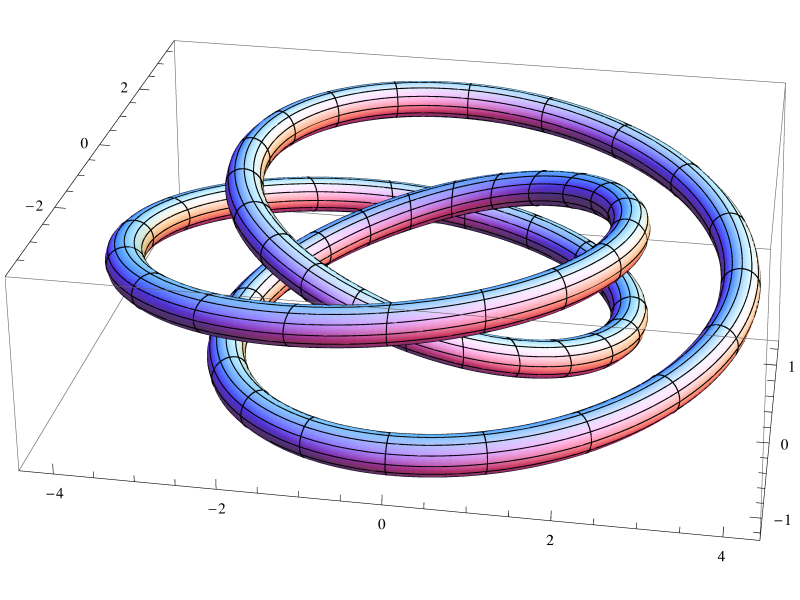
\includegraphics{KnottedTorus.png}
    }
    \caption{Verknoteter Torus}
    Quelle:  \cite{knottedtorus}
    \label{fig:knottedtorus}
\end{figure}

Dann gäbe es genau einen parallelen Schnitt durch den \cevain{cnoten}, der ein Bild wie \cref{fig:ringring} abgibt, obwohl alle \ring{ringe} und damit die Station als Ganzes ein einzelner, gewissermaßen siebenfach "`gewickelter"' Torus wäre, nämlich ein Torusknoten.

Das erklärt auch die Doppelung der Zahl $7$. Es gibt $7$ \ring{ringe} und (jeweils) $7$ \ceva{deccs}. Eine solche toroidale \ceva{cnoten}-Architektur bietet eine Erklärung für die Quasi-Identität von \ring{ringen} und \ceva{deccs}.
% Von diesen gibt es widerum verschiedene Formen, 

\paragraph{\ceva{core} als Torusknoten}

Angesichts der Bedeutung toroidaler Topologie für Fusionsreaktoren vermuten wir, dass wir hier der Topologie des \ceva{Möbius-band-accelerators} bzw. \ceva{Mino-reactors} bzw. \ceva{Cybernetischen Quecksilber-Reaktors}  auf der Spur sind (vgl.~\cref{sec:core}). \ceva{core} selber ist eine komprimierte Spiegelung der Stationsarchitektur als Ganzes. Hier entsteht durch intensive \cevain{vercnotung} die \cevain{complette verwirrung}, die für das Neuerwachen der Station nötig ist.

\paragraph{Die Raumstation als gefärbter Torusknoten}

Für jeden Torus gilt der Sieben-Farben-Satz: wie auch immer der Torus in Gebiete eingeteilt ist, es genügen genau $7$ Farben, die entstehende Landkarte einzufärben. Wir sehen hier eine topologische Begründung für die Siebenzahl der \ring{ringe}. Es könnte also eine Raumstation, deren Topologie ein (verknoteter) Torus ist, beliebig eingeteilt werden: $7$ verschiedene Kategorien von Habitaten würden genügen, um sicherzustellen, dass neben jedem Habitat ein jeweils anderes Habitat anschließt. Die Chromatische Zahl der \ceva{c-base} ist mithin ebenfalls $7$.

\begin{equation}\label{eq:chromazahl}
    \chi\left( \text{\ceva{c}}
    \right) = 7
\end{equation}

Es könnte insofern gut sein, dass $7$ \ring{ringe} eben Funktionsbereiche und nicht wirklich Kreise darstellt. 
Erschwerend kommt hinzu, dass Tori wegzusammenhängend sind; es gibt also von jedem \ring{ring} einen Weg zu jedem anderen \ring{ring}. Damit werden die wiederholten Erwähnungen von Mobilität über die \ring{ringe} hinaus bzw. zwischen ihnen plausibel.

Damit wäre die ursprüngliche Topologie ein gefärbter Torusknoten \cevain{cnoten}, mithin ein \cevain{mosaic}.

\begin{newstuff}
\lettrine{A}{n} dieser Stelle  verlassen wir  den Bereich der Empirie und begeben uns in das Reich reiner \cevain{cpeculation} bzw. purer \cevain{cience}.

Die weitere Erforschung dieser Topologie und die möglichen Ramifikationen für die energetische Effizienz des verschlungenen Miteinanders der sich ergänzenden \ring{ringe} ist eine Aufgabe ohne \cevain{endpunct}.

Uns bleibt der Hoffnung Ausdruck zu geben, dass \cevain{cünftige} Forscher die hier skizzierten Ansätze einmal zu höher Vollendung führen geworden haben werden sein können.

\ceva{vielen dank für die beachtung aller sicherheitshinweise.}
\end{newstuff}



% Und das ist ein Bild schön genug, dieses Papier zu beschließen.

% \begin{center}
%     \ceva{-- be future compatible --}    
    
%     -- be future compatible --
% \end{center}

\clearpage

\renewcommand\indexname{Fachindex}
\indexprologue{\noindent Aufgeführt sind die Stellen, an welchen Begriffe erstmalig auftauchen, sowie alle weiteren Stellen, an denen eine lateinische Umschrift mit ausgegeben wird.}
\fancyhead[RO]{Fachindex}\addcontentsline{toc}{chapter}{Fachindex}\label{sec:index}
\printindex

\clearpage

%% separate primary and secondary literature
% \chapter*{Literatur}
% \fancyhead[LO]{Literatur}\label{sec:literatur}
% \fancyhead[RO]{Primärquellen}\addcontentsline{toc}{chapter}{Literatur}
% \printbibliography[title=Primärquellen, keyword=pri,heading=subbibliography]

% \fancyhead[RO]{Weitere Quellen}\addcontentsline{toc}{chapter}{Weitere Quellen}
% \printbibliography[title=Weitere Quellen, keyword=sec,heading=subbibliography]

 
\fancyhead[LO]{Literatur}\label{sec:literatur}
\fancyhead[RO]{Literatur}\addcontentsline{toc}{chapter}{Literatur}
\printbibliography

% \clearpage
% \thispagestyle{empty}
% \vfill
% Diese \cevain{arbyte} steht unter der Lizenz \texttt{CC:BY:NC}.
% \thispagestyle{empty}
Diese \cevain{arbyte} wurde eingereicht im \cevain{ccr} zum Erlangen des Titels eines \cevain{docctor$\cdot$base}. 

Ich versichere, die vorliegende \ceva{arbyte} selbständig und eigenhändig sowie ohne unerlaubte Hilfe und ausschließlich unter Verwendung der aufgeführten \cevain{cwellen} und Hilfsmittel angefertigt zu haben. 

Ich versichere außerdem, dass die vorliegende \ceva{arbyte} noch nicht einem anderen Prüfungsverfahren zugrunde gelegen haben werden wird.

Ich erkläre mich damit einverstanden, dass diese \cevain{arbyte} unter der Lizenz \texttt{CC:BY:NC } veröffentlicht und weitergegeben werden darf.
% Ich wünsche ausdrücklich, dass sie einen Beitrag leistet für den Fortschritt der \cevain{verwirrung}.


\hfill \ceva{c-base,} \today\par
\hfill \cevain{penta}

\end{document}
